\documentclass[12pt, a4paper]{article}

% --- ESSENTIAL PACKAGES ---
\usepackage[utf8]{inputenc}
\usepackage[english]{babel}
\usepackage[T1]{fontenc}
\usepackage{graphicx}         % To insert images (e.g., ANSYS screenshots)
\usepackage{amsmath, amsfonts} % For mathematical equations
\usepackage{geometry}         % Page margins configuration
\geometry{top=2.5cm, bottom=2.5cm, left=2.5cm, right=2.5cm}
\usepackage{float}            % To force figure placement [H]
\usepackage{booktabs}         % For high-quality tables
\usepackage{xcolor}           % For text/code colors
\usepackage[hidelinks]{hyperref} % For hyperlinks and interactive table of contents
\usepackage{subcaption}
\graphicspath{{Images/}}    % Calling the Images folder

% --- HEADER AND FOOTER ---
\usepackage{fancyhdr}
\pagestyle{fancy}
\fancyhf{}
\rhead{ANSYS Simulation Project}
\lhead{Maximum Stress Analysis}
\rfoot{Page \thepage}

% --- DOCUMENT INFORMATION ---
\title{\textbf{ANSYS Numerical Simulation Report} \\ 
	\large Identification and Analysis of Maximum Stress Regions}
\author{\textbf{Written by:} Friedly WOLI}
\date{\today}

% --- BEGIN DOCUMENT ---
\begin{document}
	
	\maketitle
	
	\vspace{1cm}
	\begin{center}

		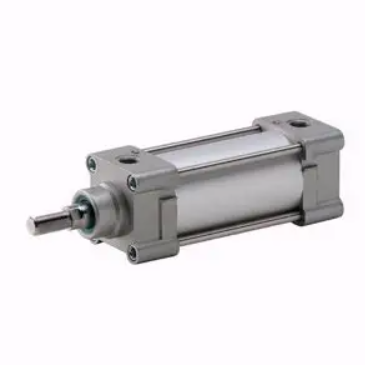
\includegraphics[width=0.7\textwidth]{real_cover.png}
	\end{center}
	
	\vfill
	
	\begin{abstract}
		This report presents a finite element simulation performed with ANSYS. The goal is to identify and analyze the maximum stress areas within the component. The boundary conditions, the meshing strategy, and the analysis of the von Mises criteria are detailed in this document.
	\end{abstract}
	
	\vfill
	\newpage
	

	
	
	%%%%%%%%%%%%%%%%%%%%%%%%%%%%%%%%%%%%%%%%%%%%%%%%%%%%%%%%%%%%%%%%%%%%%%%%%%%%%%%%%%%%%%%%%%%%%%%%%%%%%%%%%%%%%%%%%%%%%%%%
	
	%%%%%%%%%%%%%%%%%%%%%%%%%%%%%%%%%%%%%%%%%%%%%%%%%%%%%%%%%%%%%%%%%%%%%%%%%%%%%%%%%%%%%%%%%%%%%%%%%%%%%%%%%%%%%%%%%%%%%%%%
	
	
	% -----------------------------------------------------------------
	\section{Introduction and Objectives}
	% -----------------------------------------------------------------
	
	The main goal is to strenghen my understanding of structure simulation by using Ansys. To achive that gaol i will be answering cup of all questions that will lead me through all the work.
	

	
	
	
	\section{Questions Answered in the Project Report}
	\begin{itemize}
		\item What is the objective?
		\item What are the design criteria?
		\item Which quantities need to be predicted (e.g., stresses, frequency, stability)?
		\item What is the physics behind the real structure and the behavior of the modeled part?
		\item What are the available inputs?
		\item What are the requested outputs?
		\item Is it a static or dynamic problem?
		\item Is it a linear or non-linear problem?
		\item Describe the geometry.
		\item Describe the material properties.
		\item Describe the boundary conditions.
		\item Describe the meshing step.
		\item Describe the results (e.g., Von Mises stress, total deformation, equivalent strain, factor of safety).
		\item Why do you validate the simulation?
	\end{itemize}
	
	%%%%%%%%%%%%%%%%%%%%%%%%%%%%%%%%%%%%%%%%%%%%%%%%%%%%%%%%%%%%%%%%%%%%%%%%%%%%%%%%%%%%%%%%%%%%%%%%%%%%%%%%%%%%%%%%%%%%%%%%
	
	\section{Project Objectives}
	
	As mentioned in the introduction, the main goal of this project is learning. I will focus on understanding the various features of the FEA simulation software—ranging from geometry creation in DesignModeler to the meshing process, material assignment, and application of boundary conditions (such as pressures and forces). Additionally, I will investigate how different meshing techniques impact solution accuracy and analyze key output parameters, including total deformation, equivalent (Von Mises) stress, and equivalent strain, before compiling the final report.
	
	%%%%%%%%%%%%%%%%%%%%%%%%%%%%%%%%%%%%%%%%%%%%%%%%%%%%%%%%%%%%%%%%%%%%%%%%%%%%%%%%%%%%%%%%%%%%%%%%%%%%%%%%%%%%%%%%%%%%%%%%
	
	\section{Available Inputs}
	
	The analysis utilizes a specific engineering plastic with a Young's modulus of $22~\text{GPa}$ and a Poisson's ratio of $0.3$. The physical dimensions of the part are shown in Figure~\ref{fig:geo_dim}. An internal pressure of $0.5~\text{MPa}$ is applied to the inner surface of the cover. The four holes located at the corners are modeled with frictionless supports.
	
	%%%%%%%%%%%%%%%%%%%%%%%%%%%%%%%%%%%%%%%%%%%%%%%%%%%%%%%%%%%%%%%%%%%%%%%%%%%%%%%%%%%%%%%%%%%%%%%%%%%%%%%%%%%%%%%%%%%%%%%%
	
	\section{Requested Outputs}
	
	Since this is a learning-oriented project, the scope of the output analysis is broader. Key evaluation goals include:
	\begin{itemize}
		\item Analyzing the impact of material selection on final solution results.
		\item Evaluating the effects of different meshing methods and refinement levels.
		\item Investigating the distribution of stresses, deformations, and strains across the component.
	\end{itemize}
	
	%%%%%%%%%%%%%%%%%%%%%%%%%%%%%%%%%%%%%%%%%%%%%%%%%%%%%%%%%%%%%%%%%%%%%%%%%%%%%%%%%%%%%%%%%%%%%%%%%%%%%%%%%%%%%%%%%%%%%%%%
	
	\section{Static Problem Classification}
	
	The simulation is treated as a static problem due to the following factors:
	\begin{itemize}
		\item The pressure loading applied to the inner surface (shown in Figure~\ref{fig:frictionless_support}) remains constant over time.
		\item Inertial and damping effects are negligible.
		\item There are no dynamic vibrations or time-dependent loads applied to the geometry.
	\end{itemize}
	
	%%%%%%%%%%%%%%%%%%%%%%%%%%%%%%%%%%%%%%%%%%%%%%%%%%%%%%%%%%%%%%%%%%%%%%%%%%%%%%%%%%%%%%%%%%%%%%%%%%%%%%%%%%%%%%%%%%%%%%%%
	
	\section{Linearity of the Problem}
	
	The simulation is classified as linear because the stiffness matrix of the structure remains constant under the applied pressure load. Preliminary results confirm that the calculated stresses and strains do not exceed the proportional limit of the material, and small deformation theory remains valid.
	
	
	%%%%%%%%%%%%%%%%%%%%%%%%%%%%%%%%%%%%%%%%%%%%%%%%%%%%%%%%%%%%%%%%%%%%%%%%%%%%%%%%%%%%%%%%%%%%%%%%%%%%%%%%%%%%%%%%%%%%%%%%
	
	%%%%%%%%%%%%%%%%%%%%%%%%%%%%%%%%%%%%%%%%%%%%%%%%%%%%%%%%%%%%%%%%%%%%%%%%%%%%%%%%%%%%%%%%%%%%%%%%%%%%%%%%%%%%%%%%%%%%%%%%
	
	
	
	
	% -----------------------------------------------------------------
	\section{Geometric Modeling and Material Properties}
	% -----------------------------------------------------------------
	
	%%%%%%%%%%%%%%%%%%%%%%%%%%%%%%%%%%%%%%%%%%%%%%%%%%%%%%%%%%%%%%%%%%%%%%%%%%%%%%%%%%%%%%%%%%%%%%%%%%%%%%%%%%%%%%%%%%%%%%%%
	
	\subsection{Geometry}
	The geometry was modeled and imported using ANSYS DesignModeler. The lengths are made in mm.
	

	
	%%%%%%%%%%%%%%%%%%%%%%%%%%%%%%%%%%%%%%%%%%%%%%%%%%%%%%%%%%%%%%%%%%%%%%%%%%%%%%%%%%%%%%%%%%%%%%%%%%%%%%%%%%%%%%%%%%%%%%%%
	
	\subsection{Material Properties}
	The cover was initially made of an aluminum alloy. However, we will evaluate several materials to study their effect on the simulation results. those material include High-Rigidity Plastic , Standard Engineering Plastic, Lightweight Metal, Structural Metal with the characteristics listed below in Table 1. \\
	
	\begin{table}[H]
		\centering
		\caption{Mechanical properties of the material in ANSYS.}
		\label{tab:material}
		\begin{tabular}{lcc}
			\toprule
			\textbf{Property} & \textbf{Value} & \textbf{Unit} \\
			\midrule
			Young's Modulus ($E$) & $22$ & GPa \\
			Poisson's Ratio ($\nu$) & $0.3$ & -- \\
			Density ($\rho$) & $...$ & $\text{kg/m}^3$ \\
			Yield Strength ($R_e$) & $...$ & MPa \\
			\bottomrule
		\end{tabular}
	\end{table}
	
	Since we are conducting a static simulation, we only provide Young's modulus and Poisson's ratio. The other properties can be derived using the shear modulus and bulk modulus formulas: \\
	The shear modulus is $ G = \frac{E}{2(1 + \nu)} $ \\
	The bulk modulus is $ B = \frac{3 E}{1 - 2 \nu} $
	
	
	
	
	
	
	
	
	
	
	
	
	
	%%%%%%%%%%%%%%%%%%%%%%%%%%%%%%%%%%%%%%%%%%%%%%%%%%%%%%%%%%%%%%%%%%%%%%%%%%%%%%%%%%%%%%%%%%%%%%%%%%%%%%%%%%%%%%%%%%%%%%%%
	
	%%%%%%%%%%%%%%%%%%%%%%%%%%%%%%%%%%%%%%%%%%%%%%%%%%%%%%%%%%%%%%%%%%%%%%%%%%%%%%%%%%%%%%%%%%%%%%%%%%%%%%%%%%%%%%%%%%%%%%%%
	
	
	% -----------------------------------------------------------------
	\section{Boundary Conditions and Meshing}
	% -----------------------------------------------------------------
	
	%%%%%%%%%%%%%%%%%%%%%%%%%%%%%%%%%%%%%%%%%%%%%%%%%%%%%%%%%%%%%%%%%%%%%%%%%%%%%%%%%%%%%%%%%%%%%%%%%%%%%%%%%%%%%%%%%%%%%%%%
	
	\subsection{Boundary Conditions (BC)}
	The constraints and loads applied to the model are as follows:
	\begin{enumerate}
		\item \textbf{Frictionless Support:} The fixed surfaces are the internal faces of the four holes as shown in Figure \ref{frictionless_support}.
		\item \textbf{Force / Pressure:} A pressure with a magnitude of $0.5\text{ MPa}$ is applied to the internal faces as shown in Figure \ref{apply_pressure}.
	\end{enumerate}
	

	
	
	
	
	
	
	
	
	
	
	
	
	
	
	
	
	
	
	
	
	
	%%%%%%%%%%%%%%%%%%%%%%%%%%%%%%%%%%%%%%%%%%%%%%%%%%%%%%%%%%%%%%%%%%%%%%%%%%%%%%%%%%%%%%%%%%%%%%%%%%%%%%%%%%%%%%%%%%%%%%%%
	
	%%%%%%%%%%%%%%%%%%%%%%%%%%%%%%%%%%%%%%%%%%%%%%%%%%%%%%%%%%%%%%%%%%%%%%%%%%%%%%%%%%%%%%%%%%%%%%%%%%%%%%%%%%%%%%%%%%%%%%%%
	
	
	\section{Step-by-Step Mesh Study and Problem Resolution}
	
	\subsection{Step 1: Initial Setup and Problem Identification}
	The mesh was generated using default settings with a resolution of 4. Changing the resolution increased the number of nodes and elements [e.g., Tetrahedral / Hexahedral]. Local mesh refinement (\textit{Sizing}) was introduced at fillets and holes to accurately capture high stress gradients.
	
	%%%%%%%%%%%%%%%%%%%%%%%%%%%%%%%%%%%%%%%%%%%%%%%%%%%%%%%%%%%%%%%%%%%%%%%%%%%%%%%%%%%%%%%%%%%%%%%%%%%%%%%%%%%%%%%%%%%%%%%%
	
	\subsection{Step 2: Testing mesh density using global mesh controls}
	\textbf{Goal:} We are testing if simply increasing the mesh density (adding more elements/nodes) will fix high maximum stress values or bad element geometry (skewness). We increased the mesh density using global mesh controls.
	
	\textbf{Key Engineering Lesson \& Conclusion:} Increasing the mesh density, although often reducing average skewness, is not that convenient for eliminating large skewness. Increasing mesh density alone is not a panacea see picture ~\ref{fig:mesh_density_reso} . So we go for other meshing techniques.
	
	%%%%%%%%%%%%%%%%%%%%%%%%%%%%%%%%%%%%%%%%%%%%%%%%%%%%%%%%%%%%%%%%%%%%%%%%%%%%%%%%%%%%%%%%%%%%%%%%%%%%%%%%%%%%%%%%%%%%%%%%
	
	\subsection{Step 3: Testing the Patch Conforming Method}
	Patch conforming basically means meshing the face in triangles and then moving inward to create tetrahedra. This method respects the outer faces' shapes. Because of that, it is more used for complex geometry. it is also by default the meshing for complexe geometry.
	
	%%%%%%%%%%%%%%%%%%%%%%%%%%%%%%%%%%%%%%%%%%%%%%%%%%%%%%%%%%%%%%%%%%%%%%%%%%%%%%%%%%%%%%%%%%%%%%%%%%%%%%%%%%%%%%%%%%%%%%%%
	
	\subsection{Step 4: Testing the Patch Independent Method with Tetrahedrons as Method}
	We know go for independant meshing with the min size of $ 2.5mm, 3.5 mm, 6 mm $. We see that the mesh size reduce significantly from $ 2.5mm to 3 mm $ and become worse we we go to $ 6 mm$
	The opposite of patch conforming is patch independent: here, meshes are created from the inside out. In this way, the mesh exterior shape deviates from the original geometry boundary.
	
	With the patch independent method, we can see the result as the picture (\textit{name of picture}) showed us. As a result, the mesh size becomes large with around 365,174 nodes and 23,975 elements. The meshing quality is also good compared to the other methods.
	
	When we use the coarser element, the mesh size reduces to 38,452 nodes and 22,286 elements. However, when we still increase the min size limit, the quality becomes worse. It also modifies the geometry by generating distorted patches as shown in Figure \ref{fig:patch_independent}.
	

	%%%%%%%%%%%%%%%%%%%%%%%%%%%%%%%%%%%%%%%%%%%%%%%%%%%%%%%%%%%%%%%%%%%%%%%%%%%%%%%%%%%%%%%%%%%%%%%%%%%%%%%%%%%%%%%%%%%%%%%%
	
	
	\subsection{Step 5:  Testing the Patch Independent Method with Hex Dominant Method}
	Here, the mesh node count is at 35,027 and the elements count is 17,082. They increase and the mesh appears to be fine, but the quality is poor. we see that the systeme failed
	
	The idea here with hex dominant is to mesh the body with Patch Conforming first and then combine tetrahedra to form hexahedra: two tetrahedra form a hexahedron, as shown in the picture (\textit{hex\_dominant\_mth}).
	
	
	
	
	
	
	
	
	
	
	
	%%%%%%%%%%%%%%%%%%%%%%%%%%%%%%%%%%%%%%%%%%%%%%%%%%%%%%%%%%%%%%%%%%%%%%%%%%%%%%%%%%%%%%%%%%%%%%%%%%%%%%%%%%%%%%%%%%%%%%%%
	
	%%%%%%%%%%%%%%%%%%%%%%%%%%%%%%%%%%%%%%%%%%%%%%%%%%%%%%%%%%%%%%%%%%%%%%%%%%%%%%%%%%%%%%%%%%%%%%%%%%%%%%%%%%%%%%%%%%%%%%%%
		
	% -----------------------------------------------------------------
	\section{Critical Analysis and Safety Factor}
	% -----------------------------------------------------------------
	The factor of safety $s$ is calculated with respect to the yield strength $R_e$:
	\begin{equation}
		s = \frac{R_e}{\sigma_{max}} = \frac{250}{185.4} \approx 1.35
	\end{equation}
	
	Since $s > 1$, the structure remains within the elastic range and does not undergo plastic deformation under the applied load. 
	
	\textbf{Optimization Recommendations:}
	To reduce the peak stress observed at the critical location, the following design modifications are recommended:
	\begin{itemize}
		\item Increase the radius of the fillet.
		\item Locally add material near the stress hotspot.
	\end{itemize}
	
	
	
	
	
	
	
	
	
	%%%%%%%%%%%%%%%%%%%%%%%%%%%%%%%%%%%%%%%%%%%%%%%%%%%%%%%%%%%%%%%%%%%%%%%%%%%%%%%%%%%%%%%%%%%%%%%%%%%%%%%%%%%%%%%%%%%%%%%%
	
	%%%%%%%%%%%%%%%%%%%%%%%%%%%%%%%%%%%%%%%%%%%%%%%%%%%%%%%%%%%%%%%%%%%%%%%%%%%%%%%%%%%%%%%%%%%%%%%%%%%%%%%%%%%%%%%%%%%%%%%%
		
	% -----------------------------------------------------------------
	\section{Results and Maximum Stress Location}
	% -----------------------------------------------------------------
	\subsection{von Mises Stress Field}
	The solution yields the distribution of the von Mises equivalent stress $\sigma_{vm}$. The formulation for this stress criterion is expressed as:
	\begin{equation}
		\sigma_{vm} = \sqrt{\frac{1}{2} \left[ (\sigma_1 - \sigma_2)^2 + (\sigma_2 - \sigma_3)^2 + (\sigma_3 - \sigma_1)^2 \right]}
	\end{equation}
	
	%%%%%%%%%%%%%%%%%%%%%%%%%%%%%%%%%%%%%%%%%%%%%%%%%%%%%%%%%%%%%%%%%%%%%%%%%%%%%%%%%%%%%%%%%%%%%%%%%%%%%%%%%%%%%%%%%%%%%%%%
	
	\subsection{Identification of the Maximum Stress Region}
	According to the probe tools (\textit{Probe / Max}) in ANSYS:
	\begin{itemize}
		\item \textbf{Maximum stress value:} $\sigma_{max} = 185.4\text{ MPa}$.
		\item \textbf{Exact location:} The maximum stress occurs at the [e.g., inner fillet / edge of the central hole].
		\item \textbf{Physical explanation:} This area acts as a stress concentration zone caused by the abrupt geometry change.
	\end{itemize}
	
	\subsection{Total deformation}
	
	
	here i will comment the total deformation 
	
	
	\subsection{Equivalent stress}
	
	here i will comment the equivalent von mises stress
	
	
	\subsection{Strain}
	
	
	here i will comment the strain resul 
	
	
	
	
	
	
	
	
	
	
	
	
	
	%%%%%%%%%%%%%%%%%%%%%%%%%%%%%%%%%%%%%%%%%%%%%%%%%%%%%%%%%%%%%%%%%%%%%%%%%%%%%%%%%%%%%%%%%%%%%%%%%%%%%%%%%%%%%%%%%%%%%%%%
	
	%%%%%%%%%%%%%%%%%%%%%%%%%%%%%%%%%%%%%%%%%%%%%%%%%%%%%%%%%%%%%%%%%%%%%%%%%%%%%%%%%%%%%%%%%%%%%%%%%%%%%%%%%%%%%%%%%%%%%%%%
		
	\newpage
	\section{General picture }
	\subsection{geometry}
	\begin{figure}[htbp]
		\centering
		% Top Left Image
		\begin{subfigure}[b]{0.48\textwidth}
			\centering
			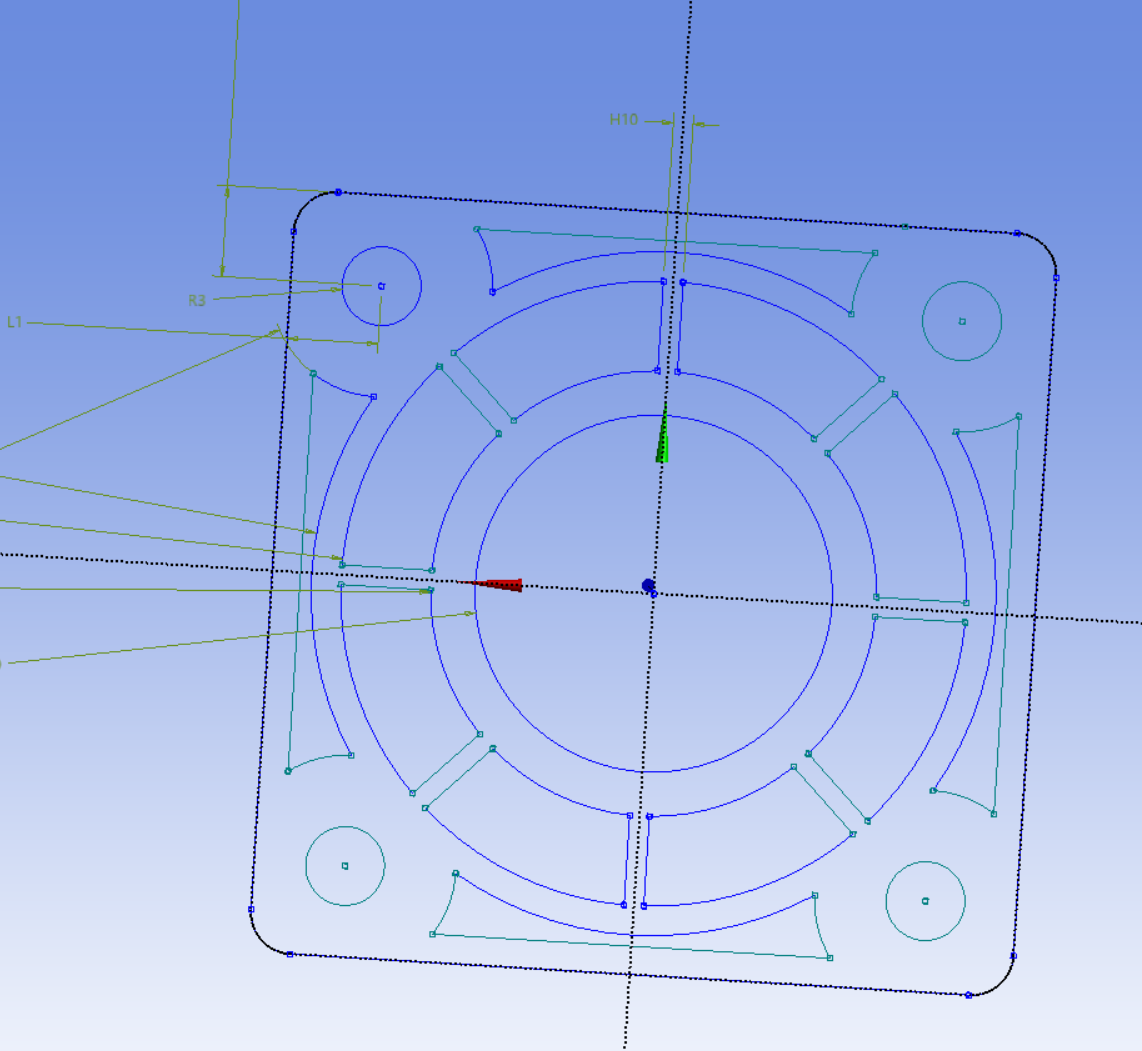
\includegraphics[width=\textwidth]{geometry_design1.png} 
			\caption{Designing of geometry}
			\label{fig:cad_geom}
		\end{subfigure}
		\hfill % Adds horizontal space between the figures
		% Top Right Image
		\begin{subfigure}[b]{0.48\textwidth}
			\centering
			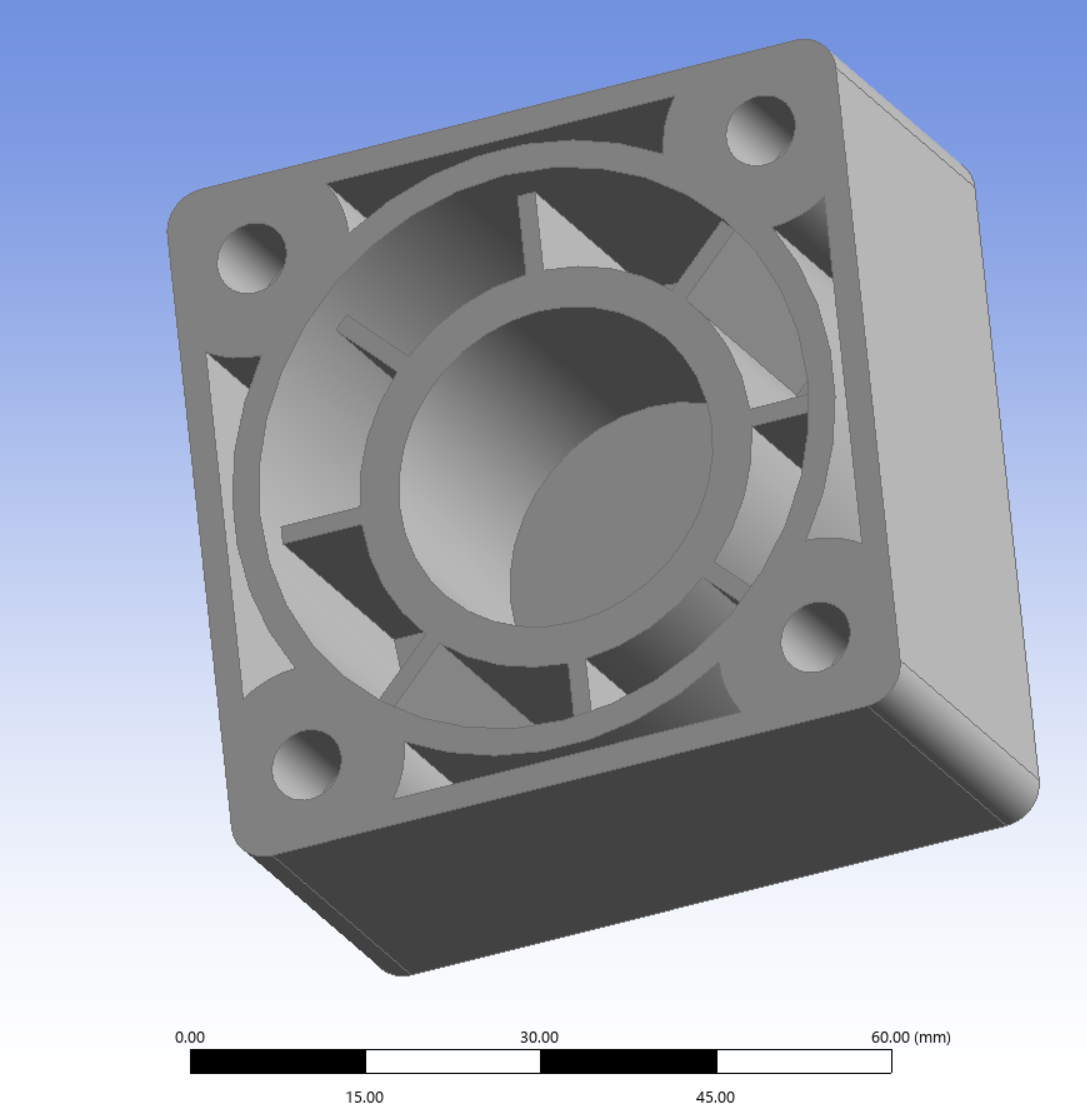
\includegraphics[width=\textwidth]{geometry1.png}
			\caption{Control volume and vehicle geometry}
			\label{fig:mesh}
		\end{subfigure}
		
		\vspace{0.5cm} % Adds vertical space between the rows
		
		% Bottom Left Image
		\begin{subfigure}[b]{0.48\textwidth}
			\centering
			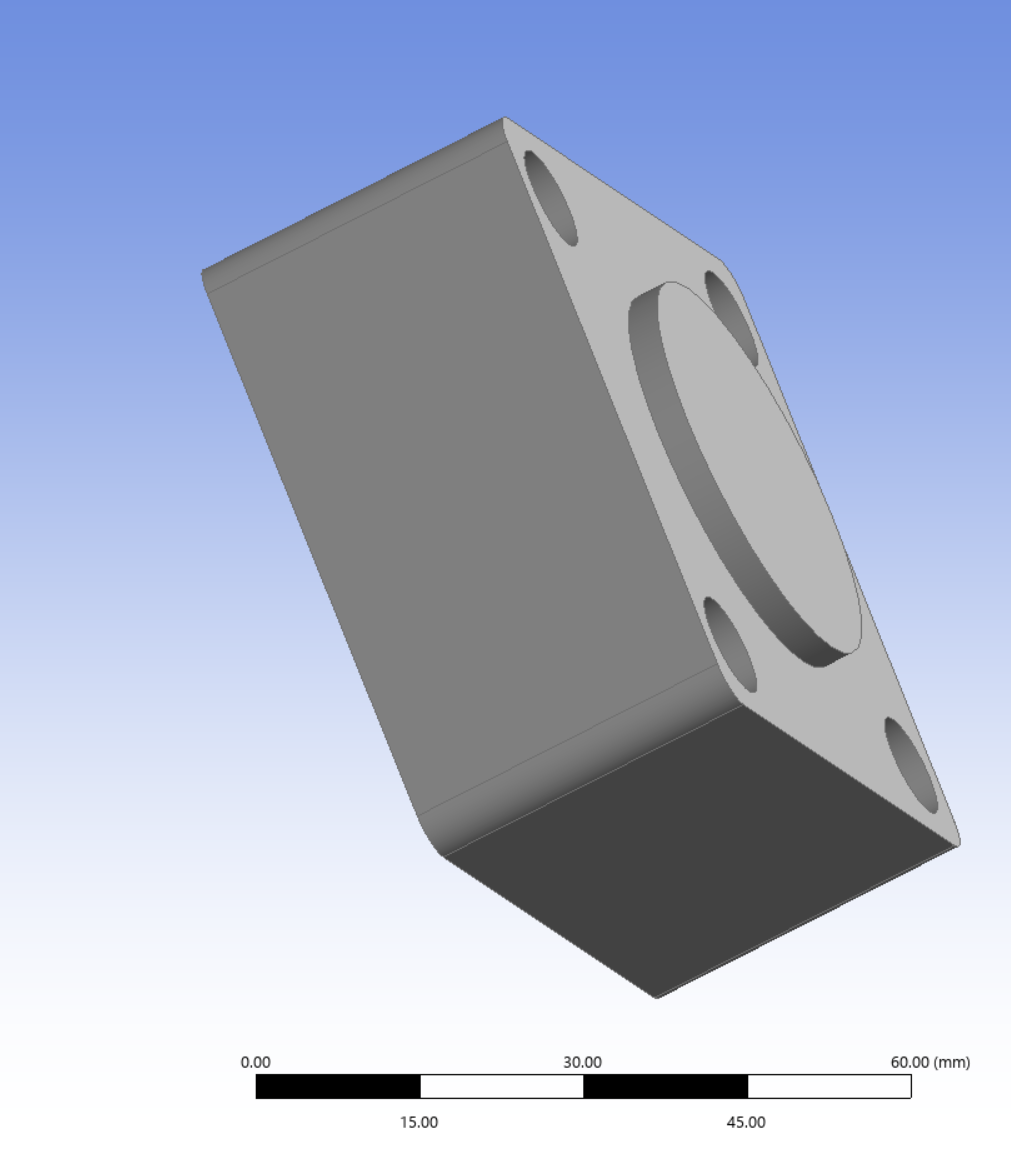
\includegraphics[width=\textwidth]{geometry2.png}
			\caption{Plane of symmetry}
			\label{fig:contour}
		\end{subfigure}
		\hfill
		% Bottom Right Image
		\begin{subfigure}[b]{0.48\textwidth}
			\centering
			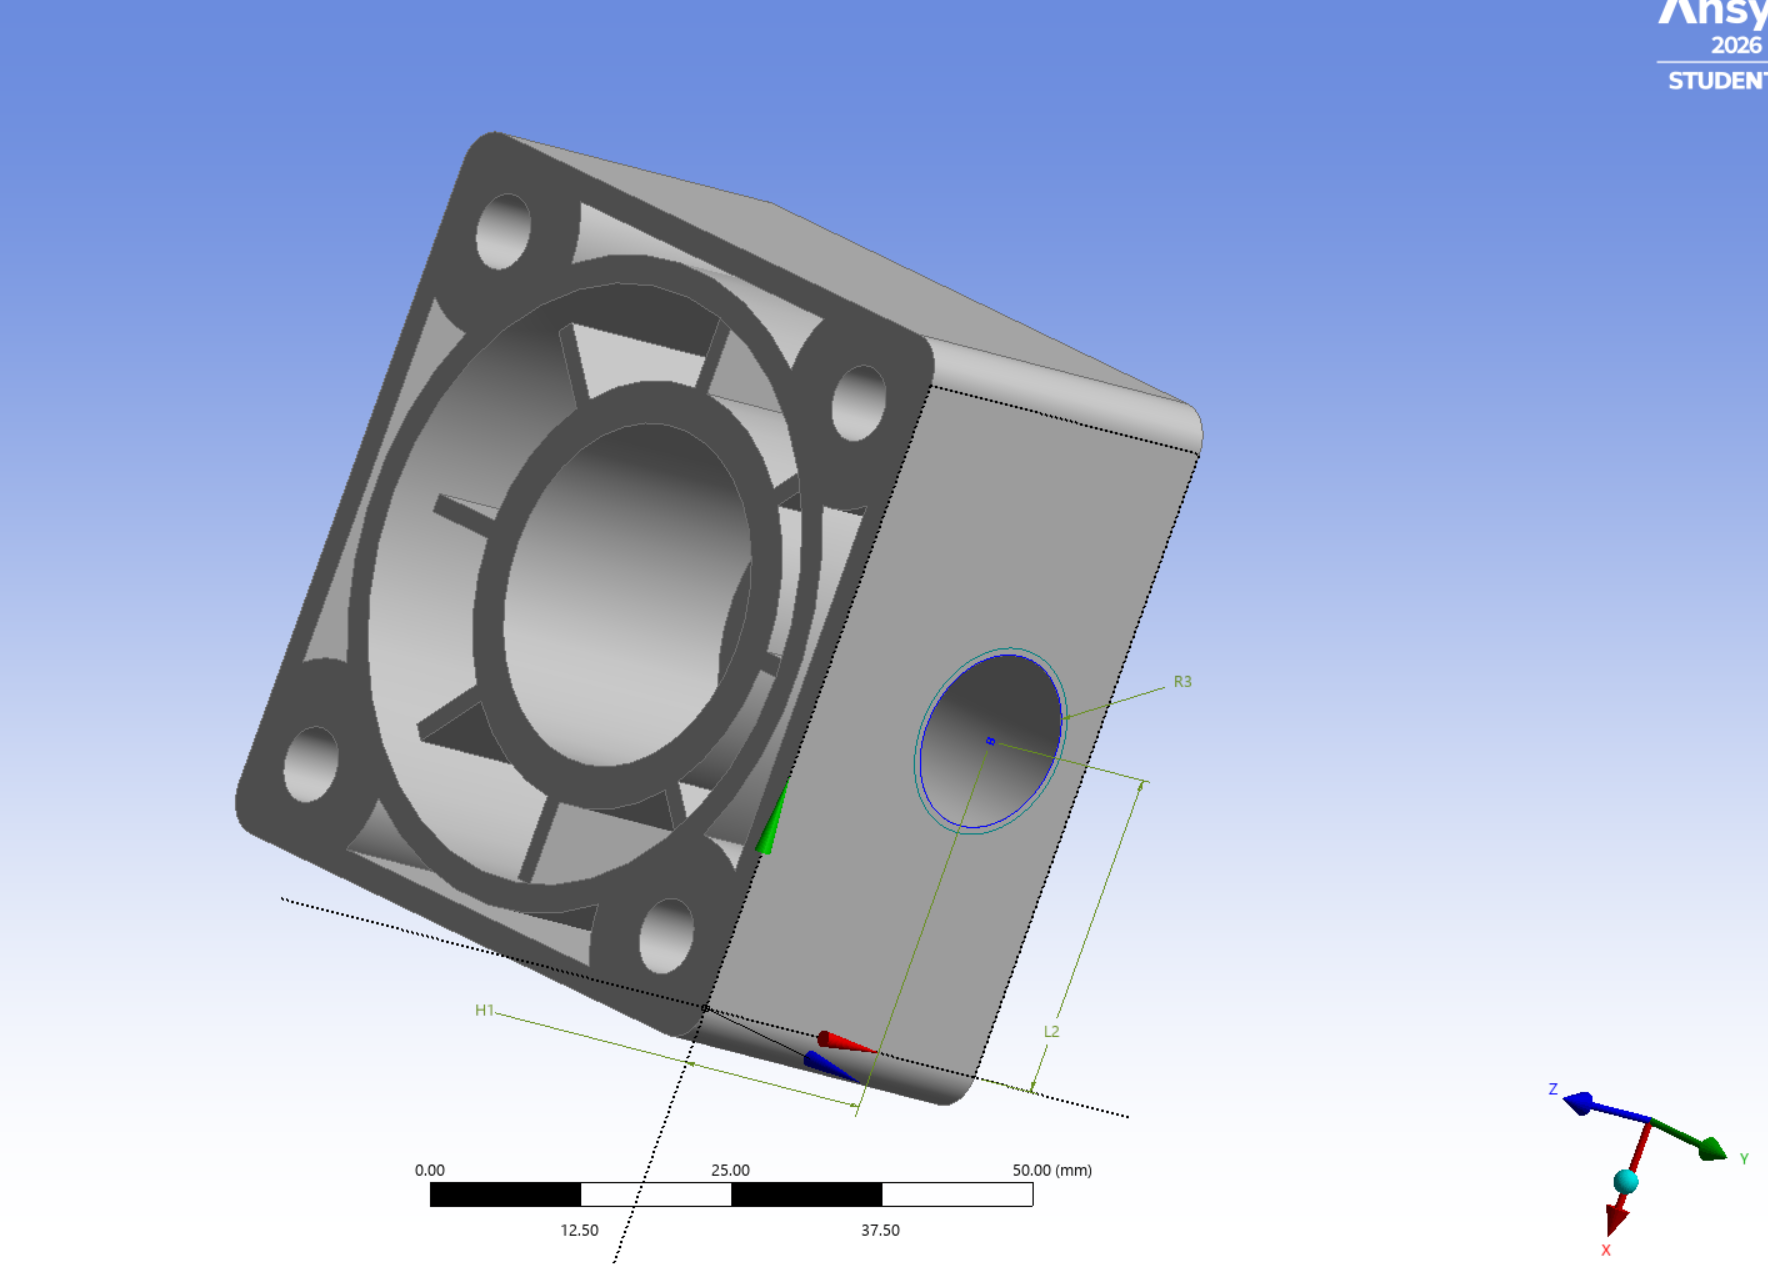
\includegraphics[width=\textwidth]{geometry4.png}
			\caption{Streamlines and wake region}
			\label{fig:wake}
		\end{subfigure}
		
		\caption{ANSYS CFD simulation Geometry design.}
		\label{fig:all_results}
	\end{figure}
	\newpage
	
		%%%%%%%%%%%%%%%%%%%%%%%%%%%%%%%%%%%%%%%%%%%%%%%%%%%%%%%%%%%%%%%%%%%%%%%%%%%%%%%%%%%%%%%%%%%%%%%%%%%%%%%%%%%%%%%%%%%%%%%%
		
	\subsection{Boundaries Condition}
	\begin{figure}[htbp]
		\centering
		% Top Left Image
		\begin{subfigure}[b]{0.48\textwidth}
			\centering
			% Replace 'cad_geometry.png' with your actual file name
			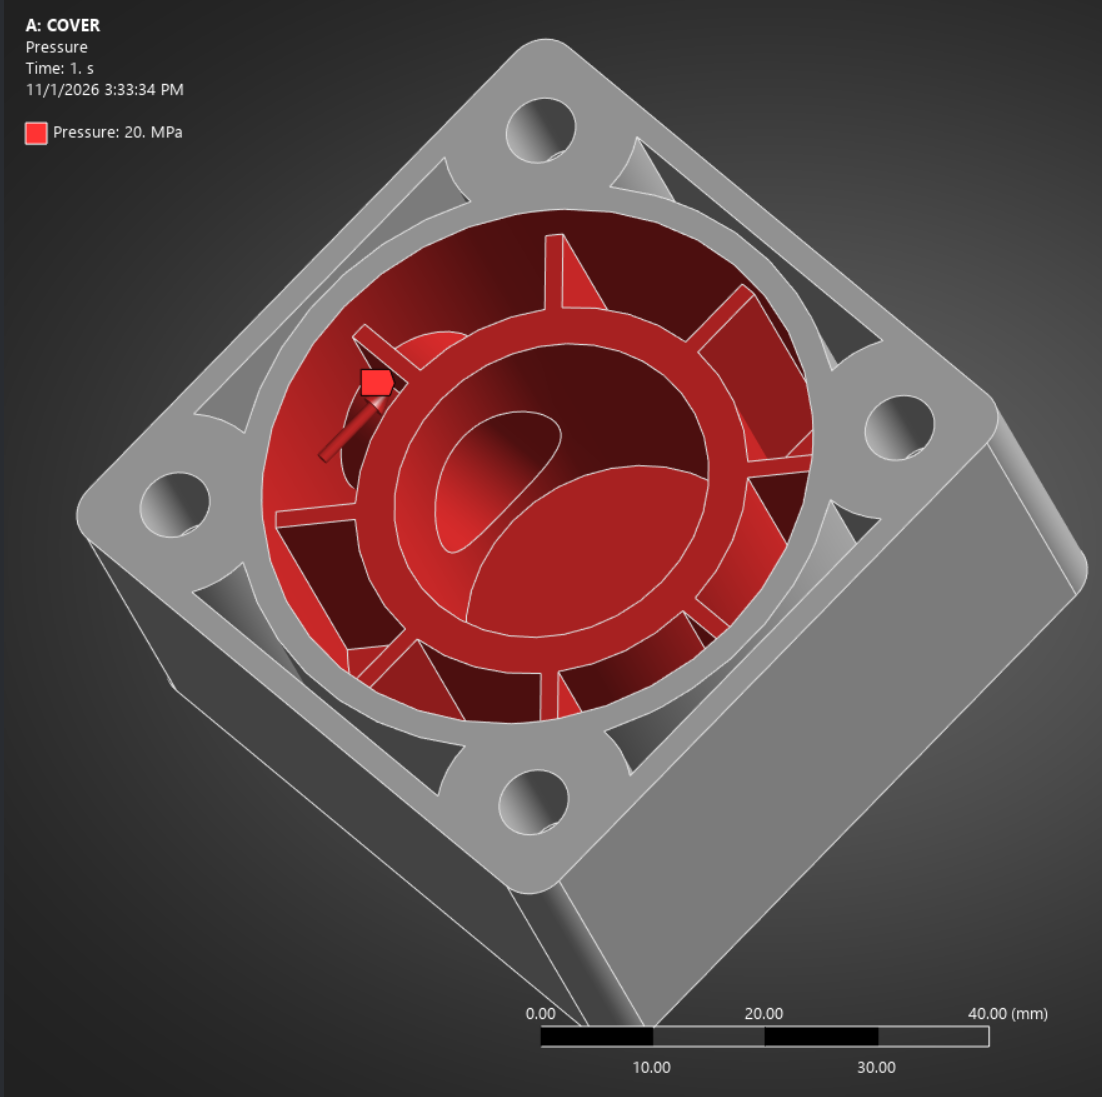
\includegraphics[width=\textwidth]{pressure_bd.png} 
			\caption{Apply pressure }
			\label{fig:cad_geom}
		\end{subfigure}
		\hfill % Adds horizontal space between the figures
		% Top Right Image
		\begin{subfigure}[b]{0.48\textwidth}
			\centering
			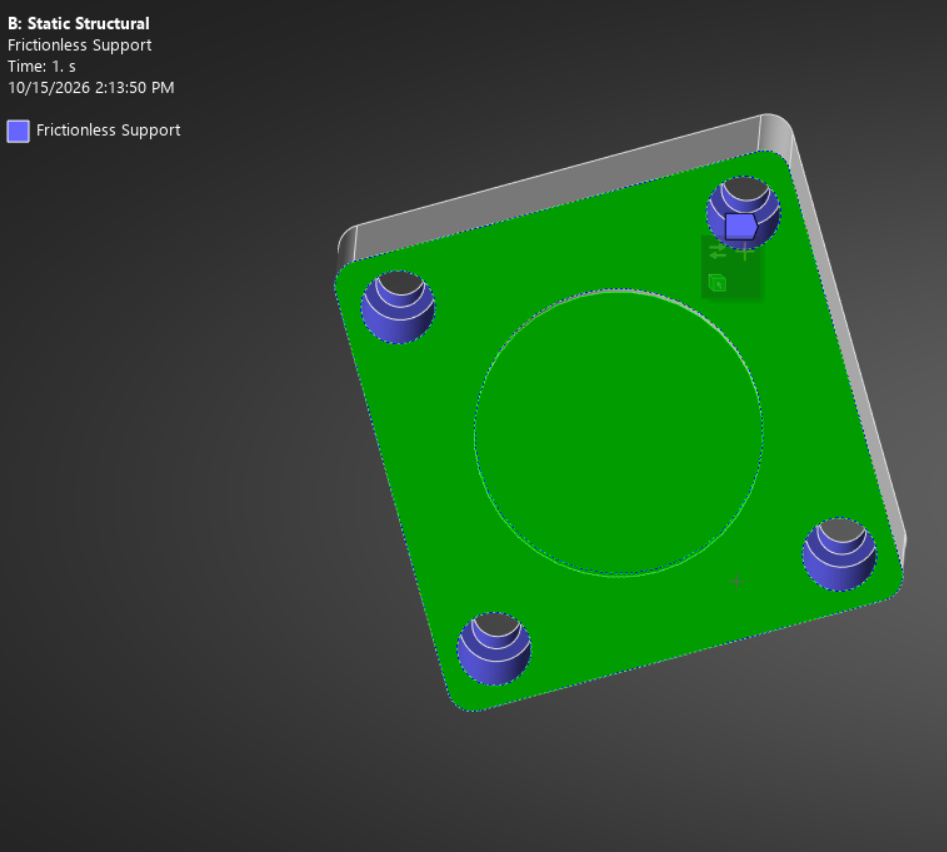
\includegraphics[width=\textwidth]{frictionless_support.png}
			\caption{Velocity contours and stagnation point}
			\label{fig:contour}
		\end{subfigure}
		
		\vspace{0.5cm} % Adds vertical space between the rows
		
		\caption{ANSYS CFD simulation Boundary condition.}
		\label{fig:all_results}
	\end{figure}
	\newpage
	
	
	
		%%%%%%%%%%%%%%%%%%%%%%%%%%%%%%%%%%%%%%%%%%%%%%%%%%%%%%%%%%%%%%%%%%%%%%%%%%%%%%%%%%%%%%%%%%%%%%%%%%%%%%%%%%%%%%%%%%%%%%%%
	
	
	
	\subsection{Meshing}
	
	The goal here is to have a look at some mesching techniques
	
	
	\begin{figure}[htbp]
		\centering
		% Top Left Image
		\begin{subfigure}[b]{0.48\textwidth}
			\centering
			% Replace 'cad_geometry.png' with your actual file name
			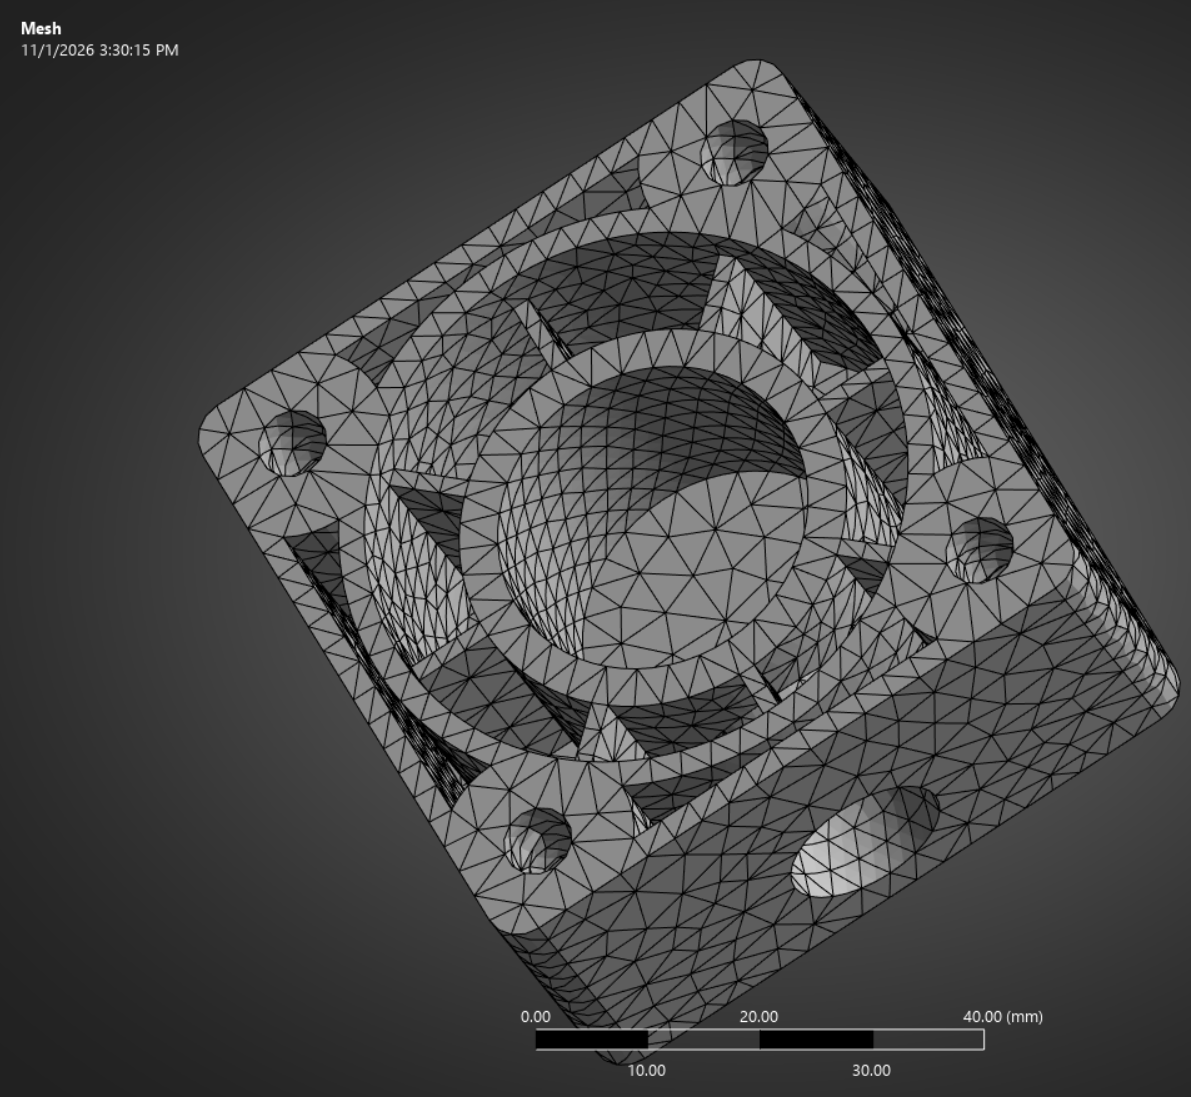
\includegraphics[width=\textwidth]{meshing1.png} 
			\caption{Default meshing }
			\label{fig:default_meshing}
		\end{subfigure}
		\hfill % Adds horizontal space between the figures
		% Top Right Image
		\begin{subfigure}[b]{0.48\textwidth}
			\centering
			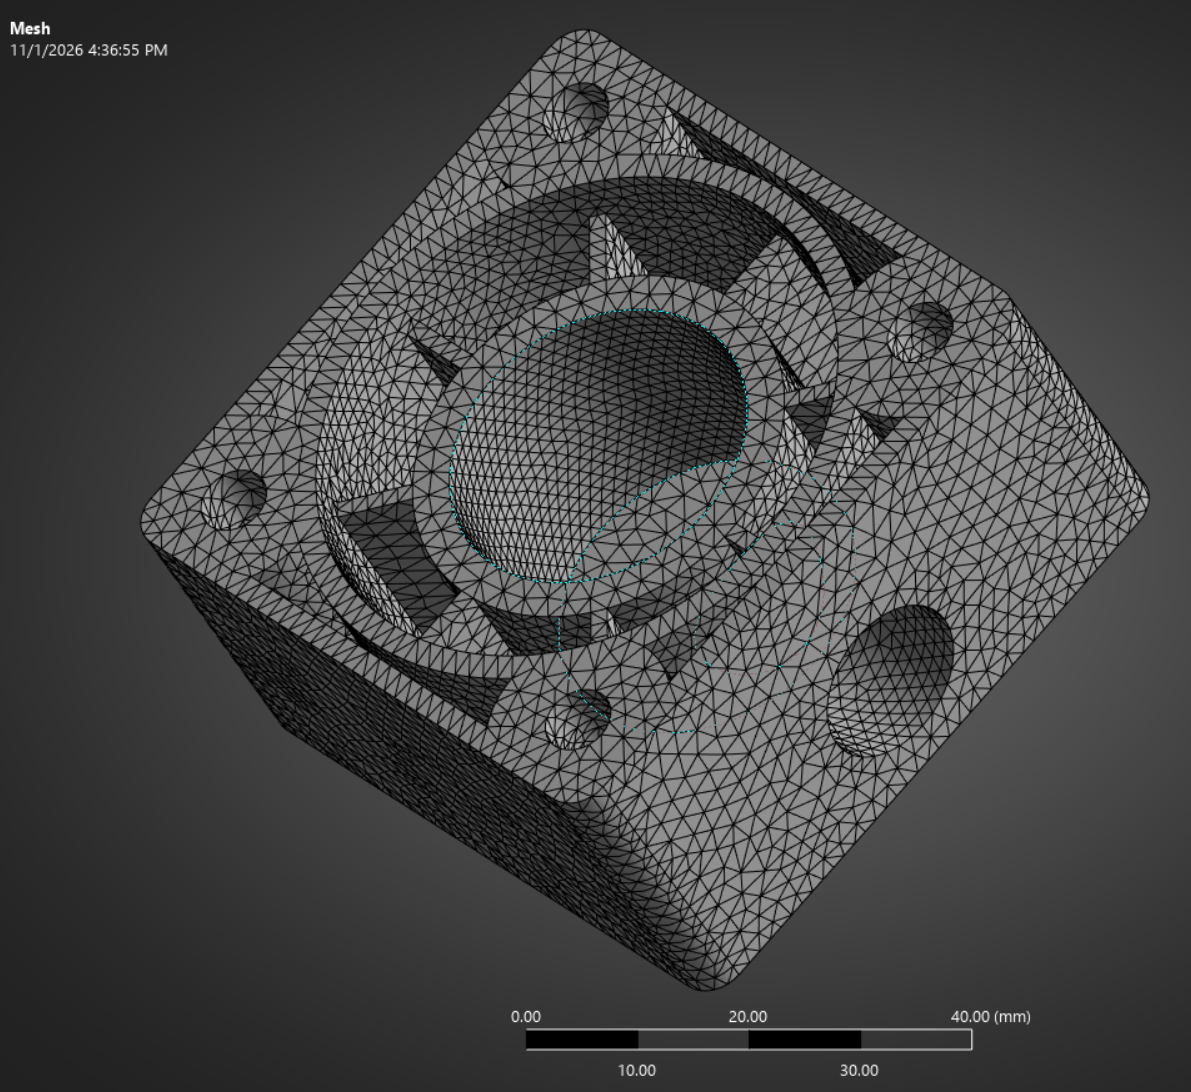
\includegraphics[width=\textwidth]{mesh_density_reso_6.png}
			\caption{Mesh density with resolution 6 and skewness}
			\label{fig:mesh_density_reso}
		\end{subfigure}
		
		\vspace{0.5cm} % Adds vertical space between the rows
		
		% Bottom Left Image
		\begin{subfigure}[b]{0.48\textwidth}
			\centering
			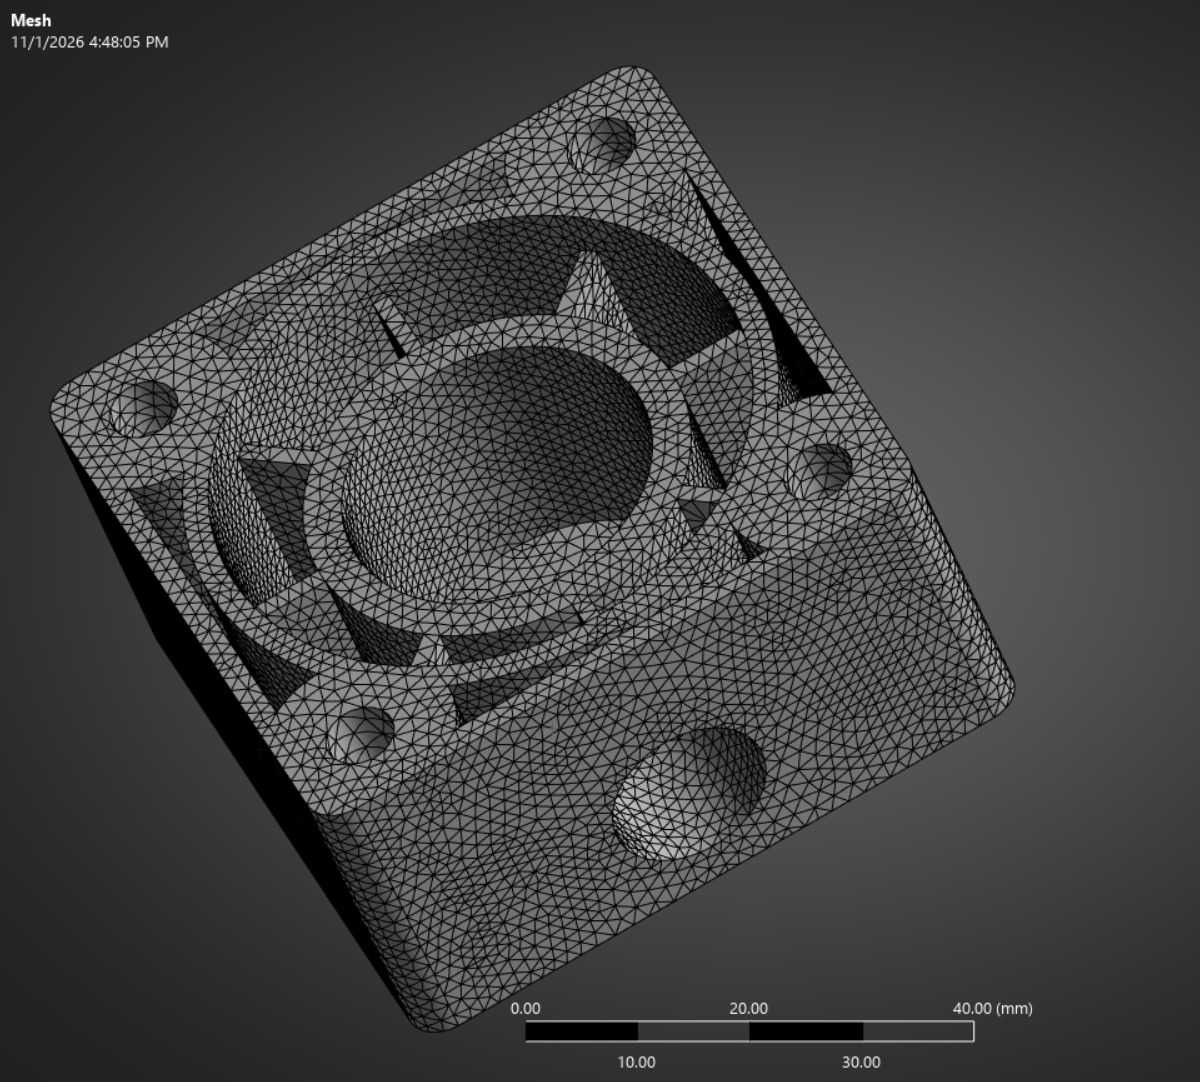
\includegraphics[width=\textwidth]{meshin_patch_independent_minsize_2.5mm.png}
			\caption{Meshing with Patch independent }
			\label{fig:meshin_patch_independent_minsize_2.5mm}
		\end{subfigure}
		\hfill
		% Bottom Right Image
		\begin{subfigure}[b]{0.48\textwidth}
			\centering
			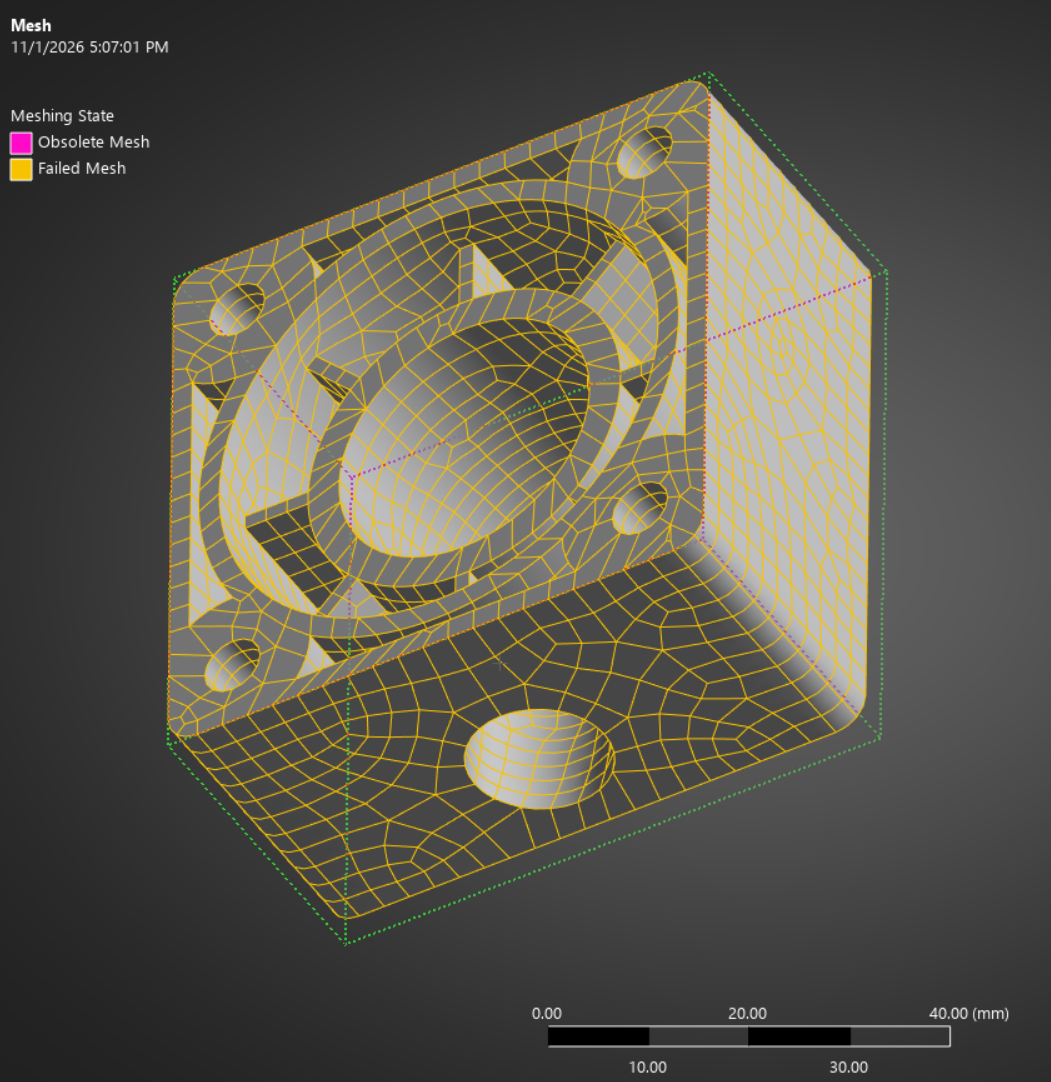
\includegraphics[width=\textwidth]{meshin_patch_independent_hex_dominant_mth.png}
			\caption{Streamlines and wake region}
			\label{fig:meshin_patch_independent_hex_dominant_mth}
		\end{subfigure}
		
	
	\end{figure}


		\newpage
		
		
		
		\begin{figure}[htbp]
			\centering
			% Top Left Image
			\begin{subfigure}[b]{0.48\textwidth}
				\centering
				% Replace 'cad_geometry.png' with your actual file name
				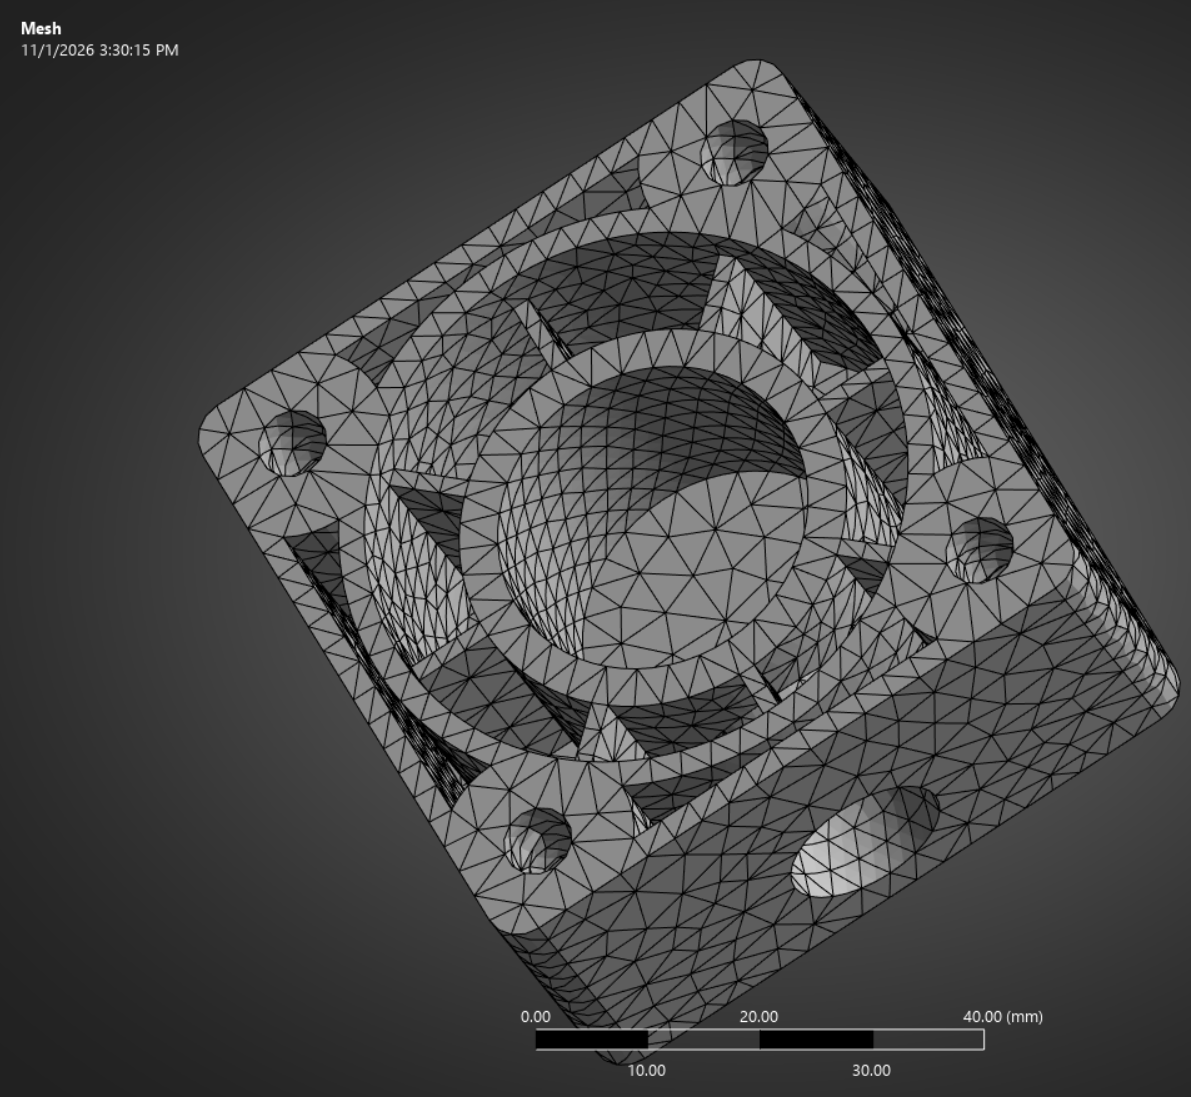
\includegraphics[width=\textwidth]{meshing1.png} 
				\caption{Default meshing }
				\label{fig:default_meshing}
			\end{subfigure}
			\hfill % Adds horizontal space between the figures
			% Top Right Image
			\begin{subfigure}[b]{0.48\textwidth}
				\centering
				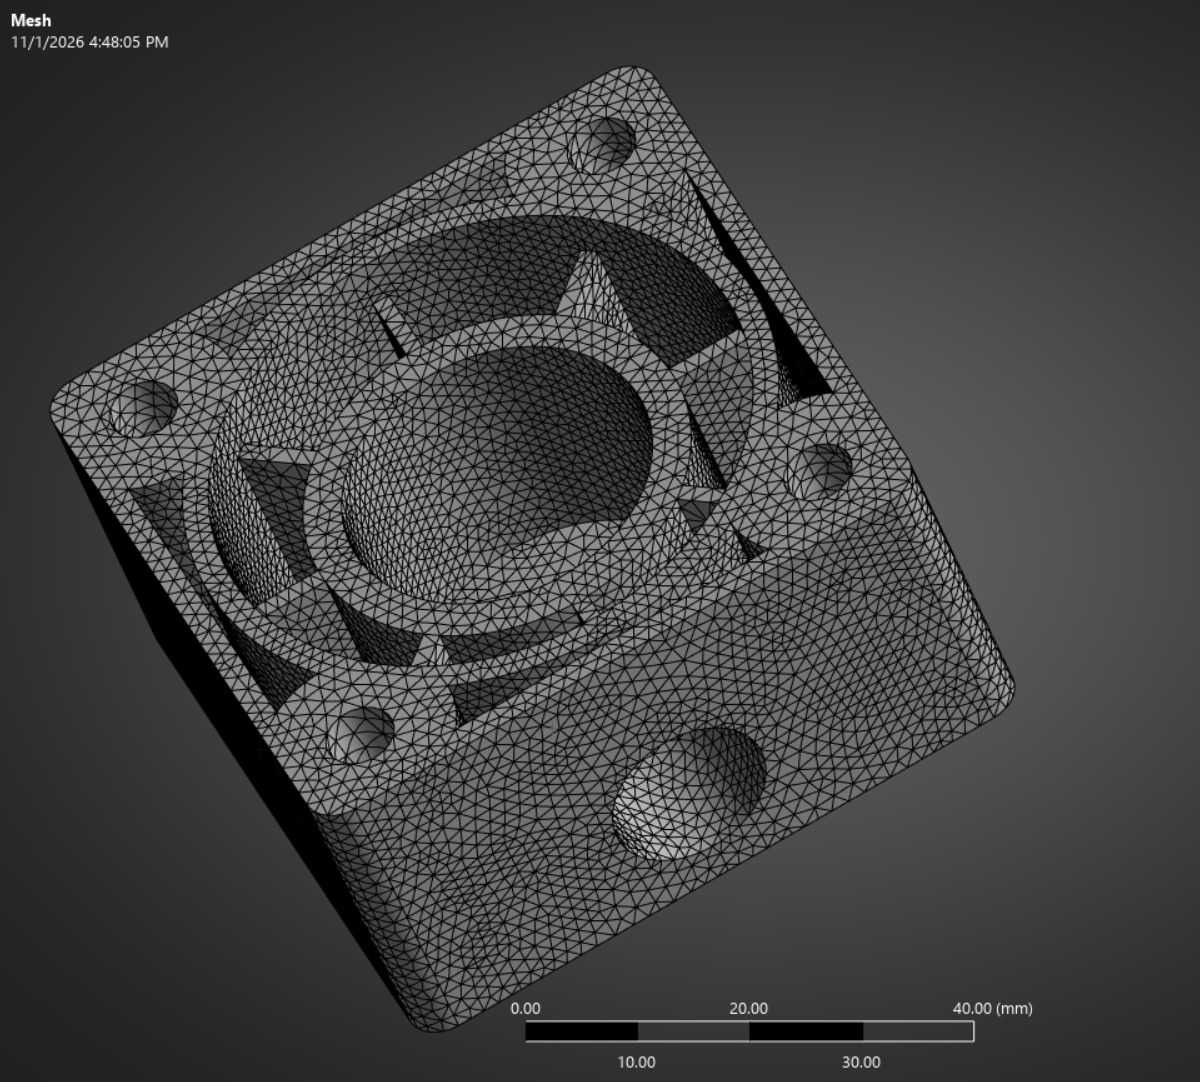
\includegraphics[width=\textwidth]{meshin_patch_independent_minsize_2.5mm.png}
				\caption{Meshing with Patch independent with a min size of 2.5 mm}
				\label{fig:meshin_patch_independent_minsize_2.5mm}
			\end{subfigure}
			
			\vspace{0.5cm} % Adds vertical space between the rows
			
			% Bottom Left Image
			\begin{subfigure}[b]{0.48\textwidth}
				\centering
				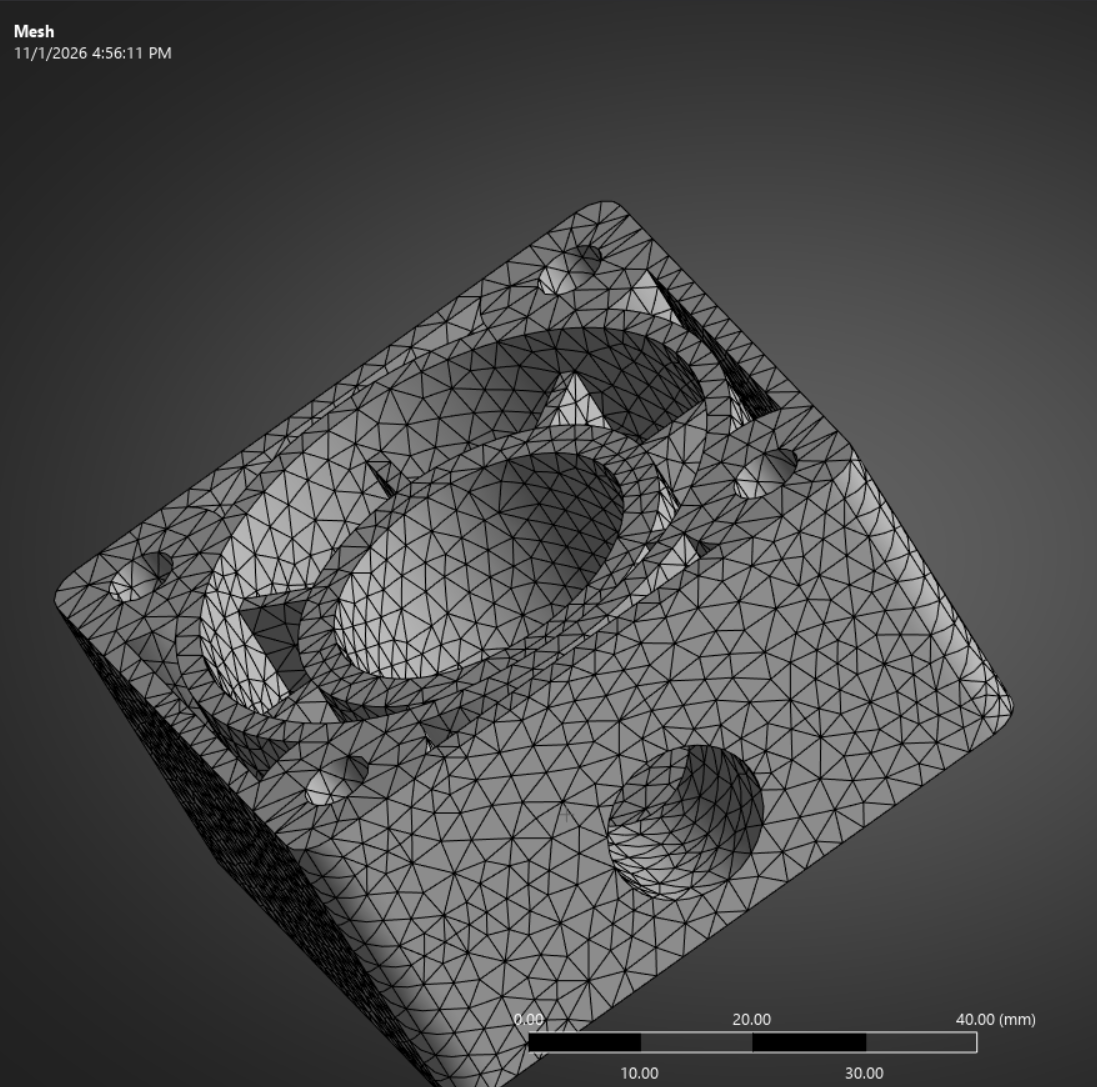
\includegraphics[width=\textwidth]{meshin_patch_independent_minsize_3mm.png}
				\caption{Meshing with Patch independent with a min size of 3 mm }
				\label{fig:meshin_patch_independent_minsize_3mm}
			\end{subfigure}
			\hfill
			% Bottom Right Image
			\begin{subfigure}[b]{0.48\textwidth}
				\centering
				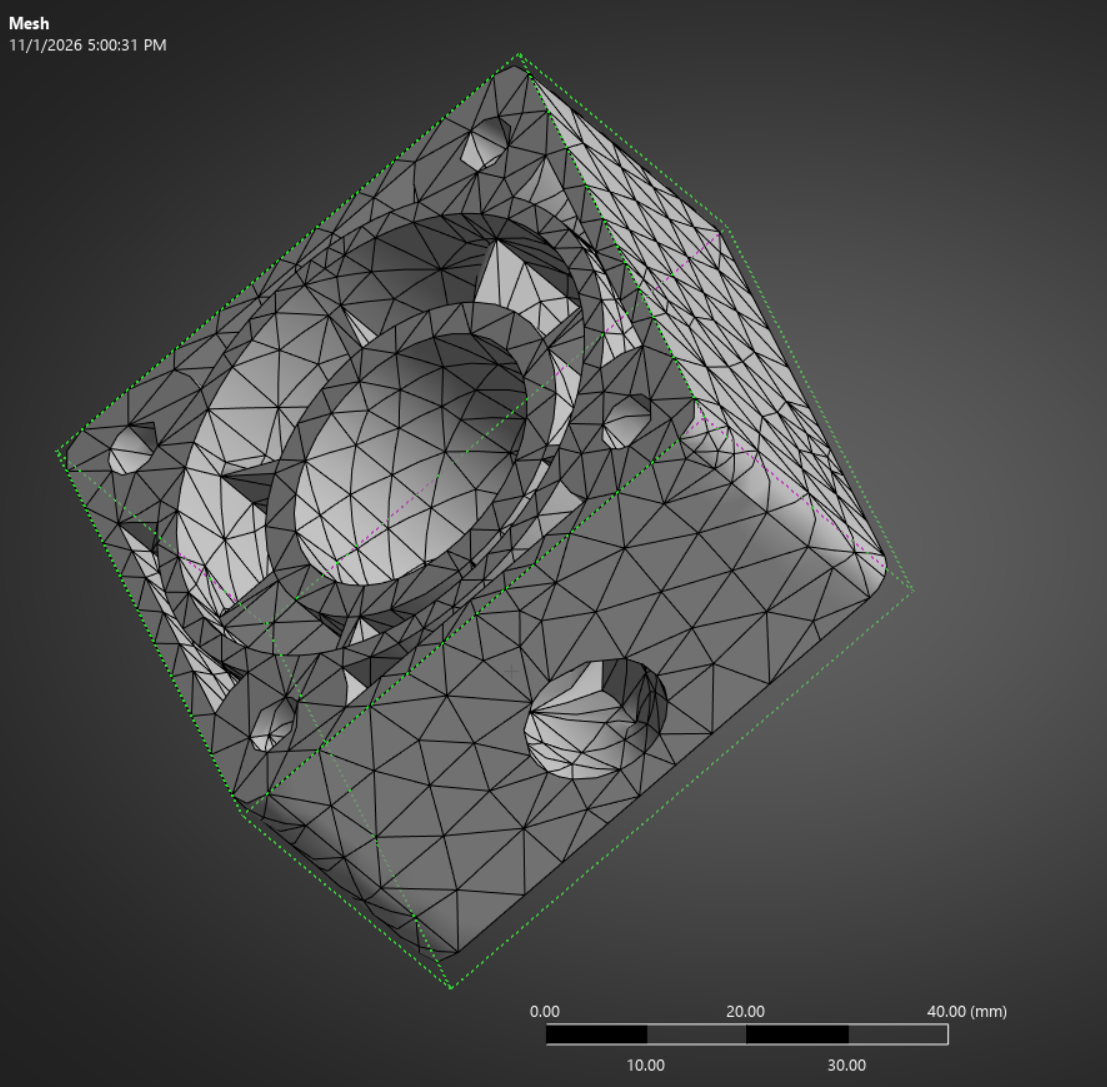
\includegraphics[width=\textwidth]{meshin_patch_independent_minsize_6mm.png}
				\caption{Meshing with Patch independent with a min size of 6 mm}
				\label{fig:meshin_patch_independent_minsize_6mm}
			\end{subfigure}
			
			\caption{ANSYS CFD simulation meshing result.}
			\label{fig:all_results}
		\end{figure}


		\newpage

	%%%%%%%%%%%%%%%%%%%%%%%%%%%%%%%%%%%%%%%%%%%%%%%%%%%%%%%%%%%%%%%%%%%%%%%%%%%%%%%%%%%%%%%%%%%%%%%%%%%%%%%%%%%%%%%%%%%%%%%%
	
	\subsection{Results}
		\subsubsection{Total deformation}
		\begin{figure}[htbp]
			\centering
			% Top Left Image
			\begin{subfigure}[b]{0.48\textwidth}
				\centering
				% Replace 'cad_geometry.png' with your actual file name
				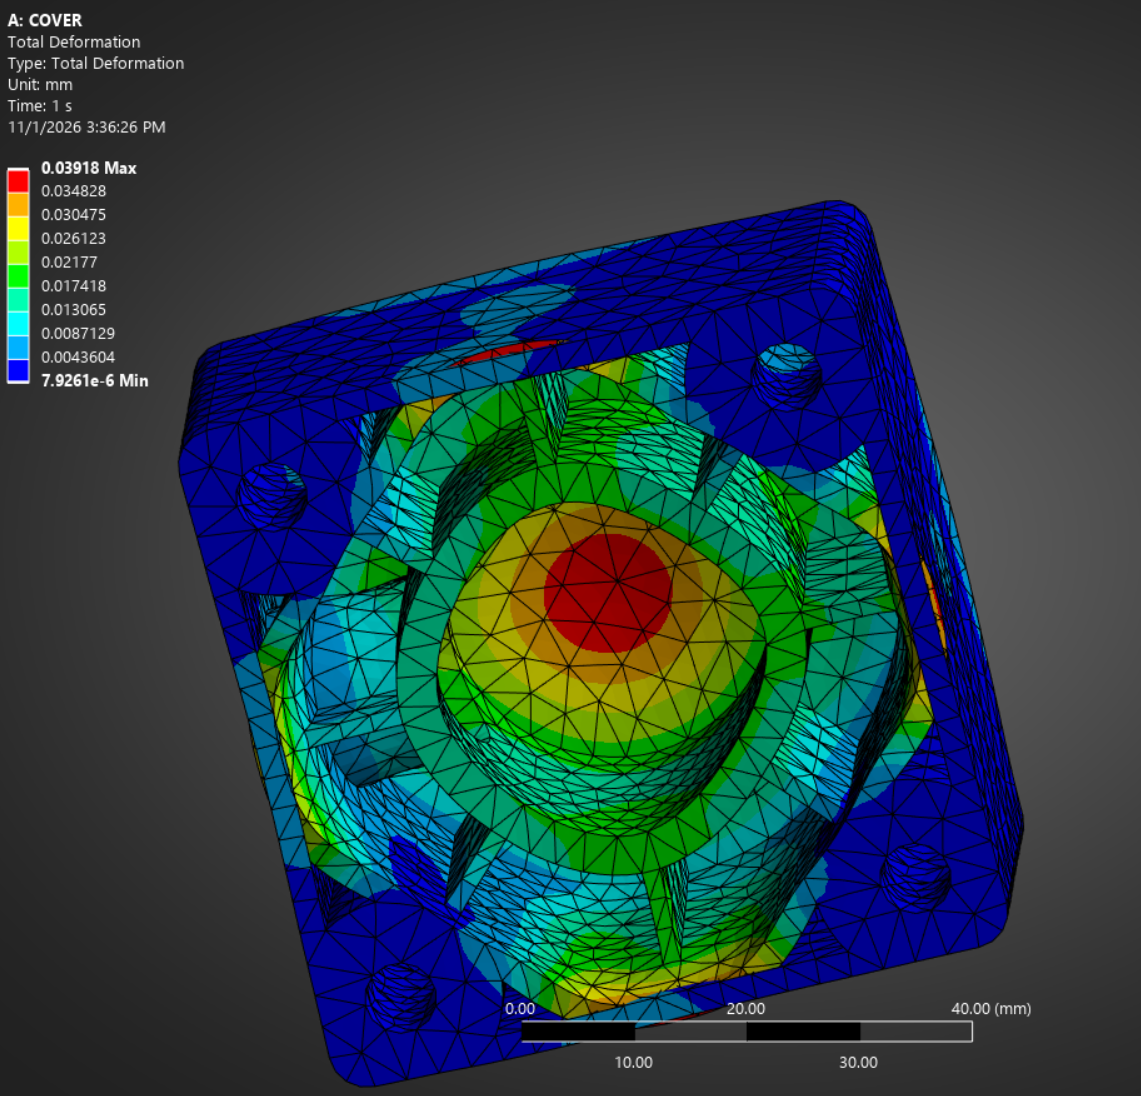
\includegraphics[width=\textwidth]{total_deformation.png} 
				\caption{Total deformation}
				\label{fig:cad_geom}
			\end{subfigure}
			\hfill % Adds horizontal space between the figures
			% Top Right Image
			\begin{subfigure}[b]{0.48\textwidth}
				\centering
				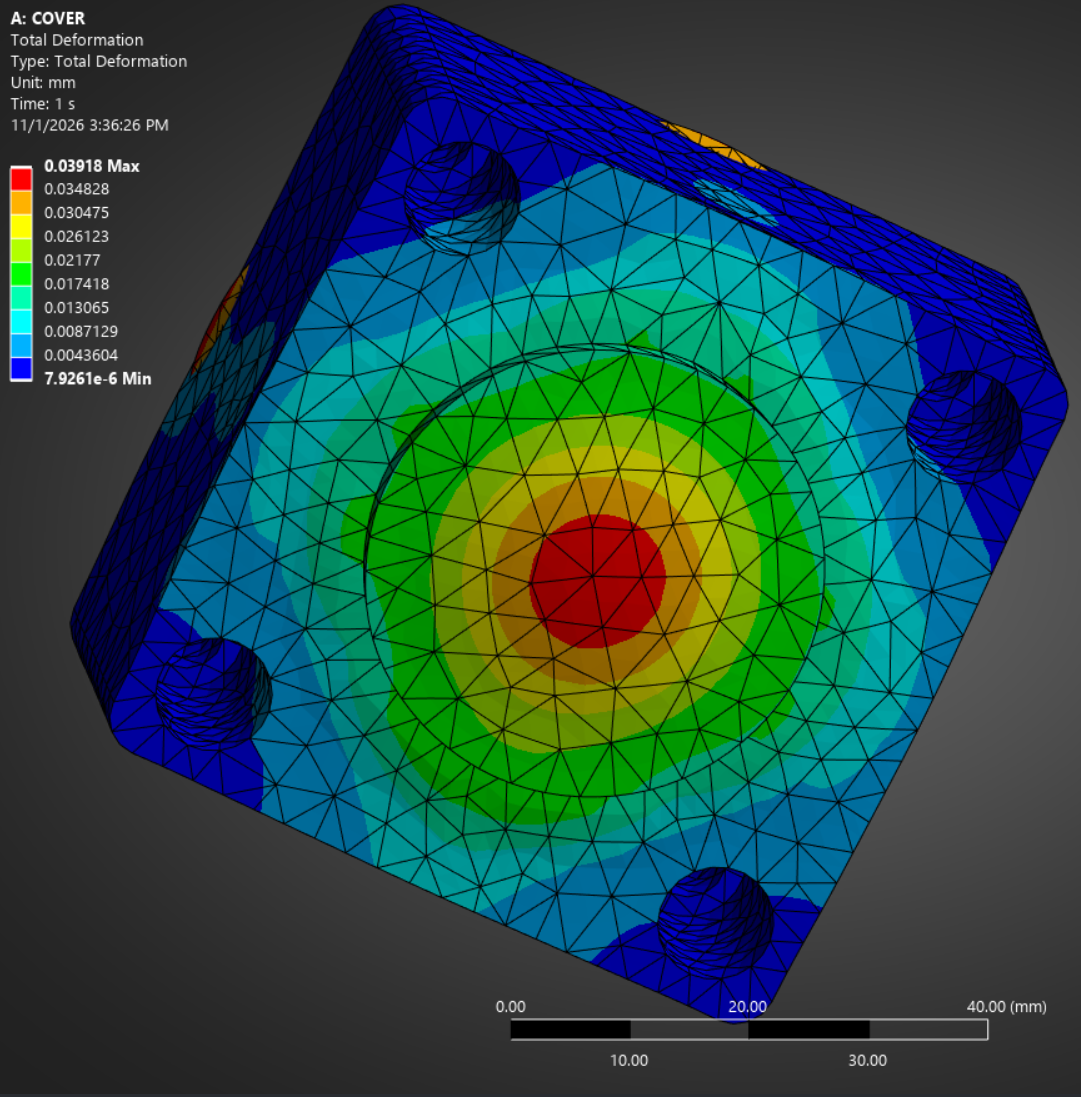
\includegraphics[width=\textwidth]{total_deformation1.png}
				\caption{Total deformation on the under surface}
				\label{fig:mesh}
			\end{subfigure}
			
			\vspace{0.5cm} % Adds vertical space between the rows
			
			% Bottom Left Image
			\begin{subfigure}[b]{0.48\textwidth}
				\centering
				%\includegraphics[width=\textwidth]{velocity_contour.png}
				\caption{Velocity contours and stagnation point}
				\label{fig:contour}
			\end{subfigure}
			\hfill
			% Bottom Right Image
			\begin{subfigure}[b]{0.48\textwidth}
				\centering
				%\includegraphics[width=\textwidth]{streamlines_wake.png}
				\caption{Streamlines and wake region}
				\label{fig:wake}
		\end{subfigure}
		
		\caption{ANSYS CFD simulation Total deformation.}
		\label{fig:all_results}
		
		\end{figure}
				\newpage
	%%%%%%%%%%%%%%%%%%%%%%%%%%%%%%%%%%%%%%%%%%%%%%%%%%%%%%%%%%%%%%%%%%%%%%%%%%%%%
			
		\subsubsection{Equivalent stress}	
		\begin{figure}[htbp]
			\centering
			% Top Left Image
			\begin{subfigure}[b]{0.48\textwidth}
				\centering
				% Replace 'cad_geometry.png' with your actual file name
				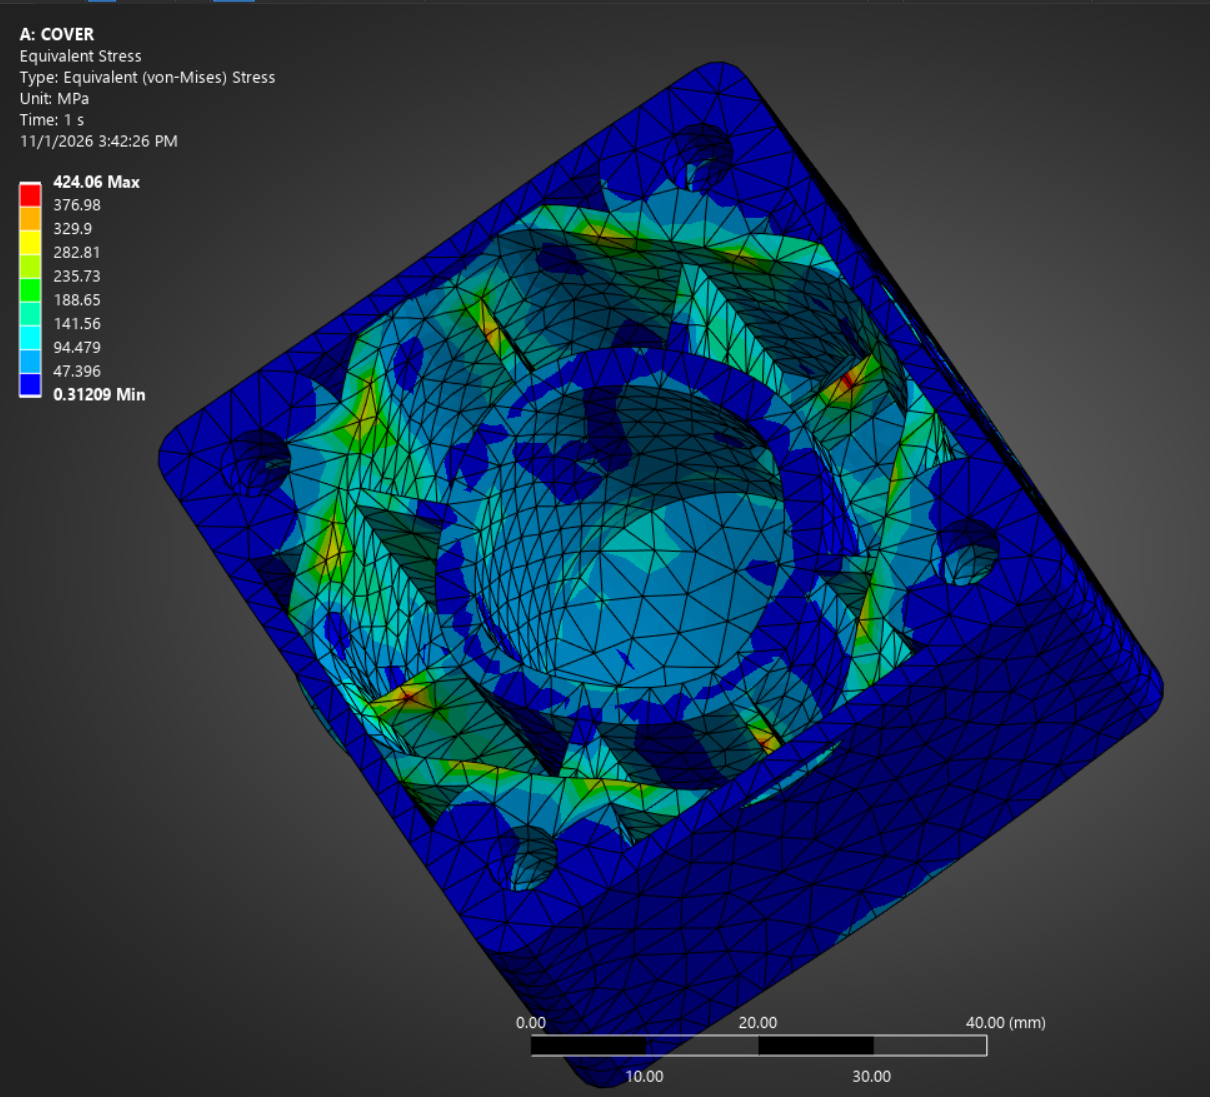
\includegraphics[width=\textwidth]{equivalent_stress1.png} 
				\caption{Equivalent stress }
				\label{fig:cad_geom}
			\end{subfigure}
			\hfill % Adds horizontal space between the figures
			% Top Right Image
			\begin{subfigure}[b]{0.48\textwidth}
				\centering
				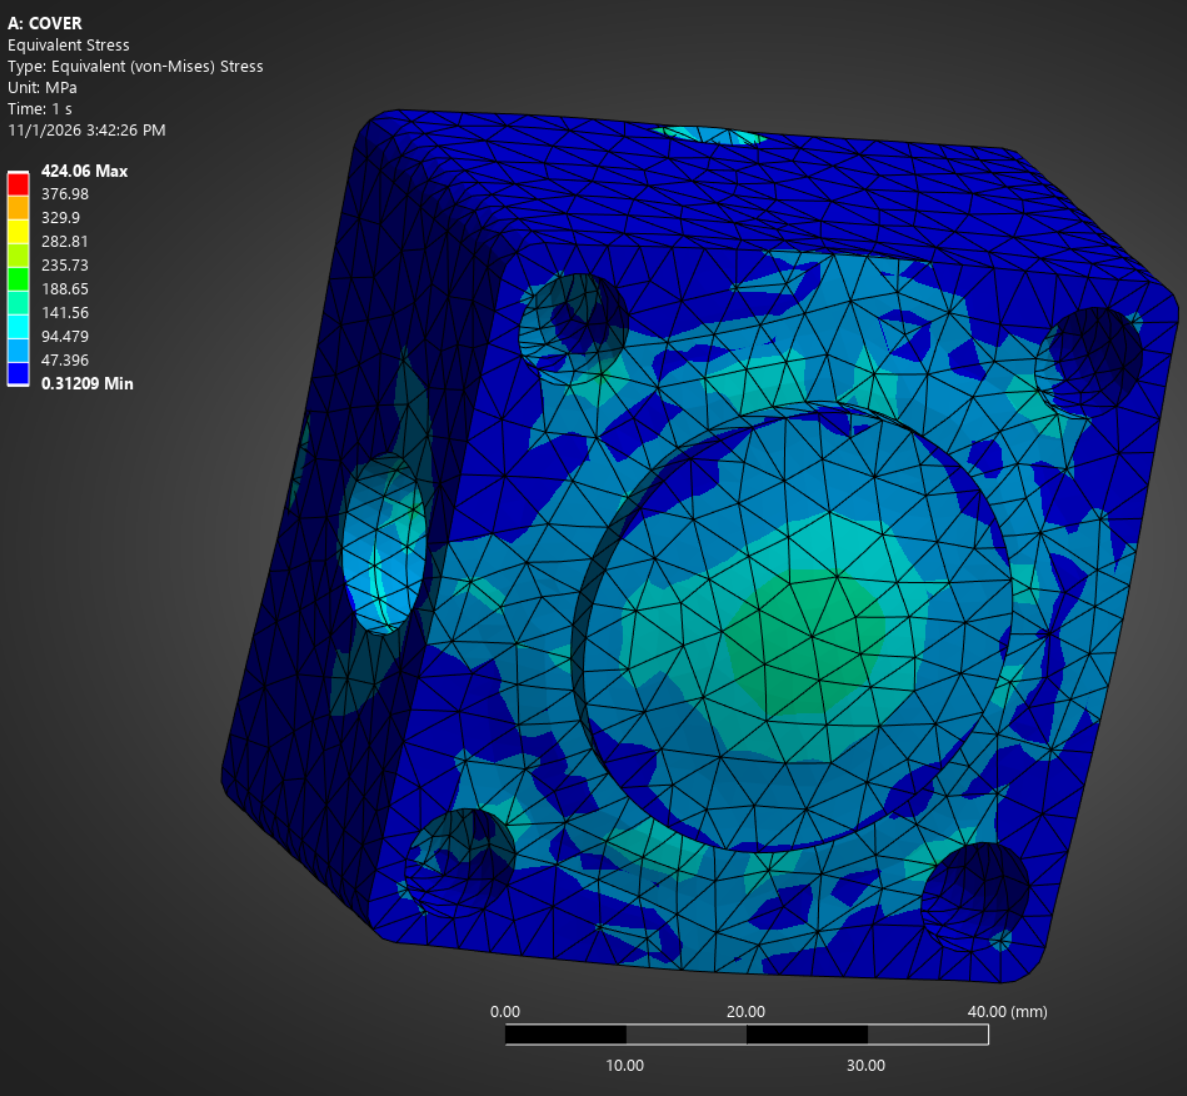
\includegraphics[width=\textwidth]{equivalent_stress2.png}
				\caption{Equvalent stress on under surface}
				\label{fig:mesh}
			\end{subfigure}
			
			\vspace{0.5cm} % Adds vertical space between the rows
			
			% Bottom Left Image
			\begin{subfigure}[b]{0.48\textwidth}
				\centering
				%\includegraphics[width=\textwidth]{starin1.png}
				\caption{Velocity contours and stagnation point}
				\label{fig:contour}
			\end{subfigure}
			\hfill
			% Bottom Right Image
			\begin{subfigure}[b]{0.48\textwidth}
				\centering
				%\includegraphics[width=\textwidth]{streamlines_wake.png}
				\caption{Streamlines and wake region}
				\label{fig:wake}
			\end{subfigure}
		
		\caption{ANSYS CFD simulation Equivalent stress}
		\label{fig:all_results}
		
		\end{figure}
			
				\newpage
				%%%%%%%%%%%%%%%%%%%%%%%%%%%%%%%%%%%%%%%%%%%%%%%%%%%%%%%%%%%%%%%%%%%%
		\subsubsection{Strain}
		\begin{figure}[htbp]
			\centering
			% Top Left Image
			\begin{subfigure}[b]{0.48\textwidth}
				\centering
				% Replace 'cad_geometry.png' with your actual file name
				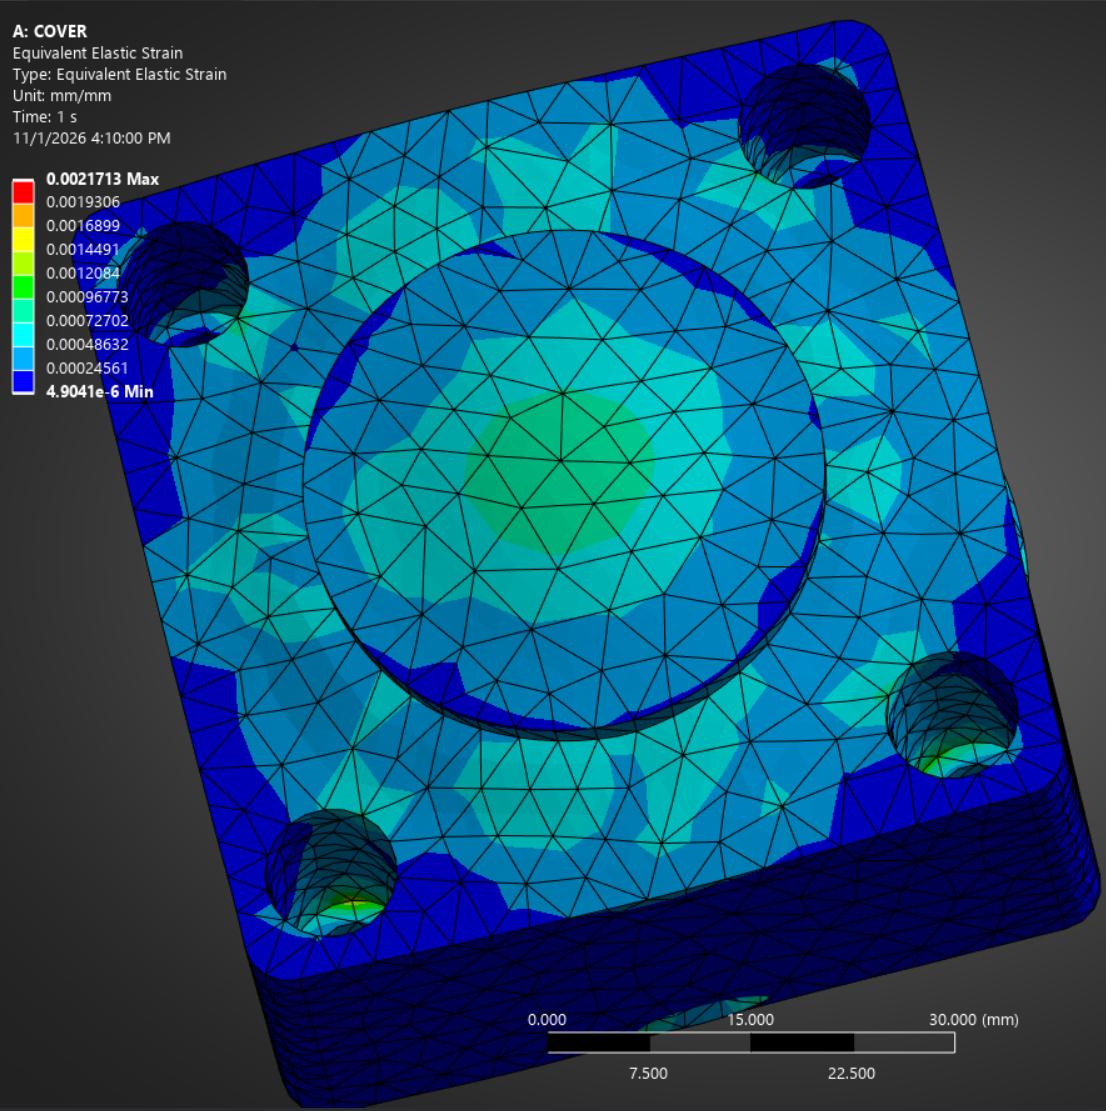
\includegraphics[width=\textwidth]{strain1.png} 
				\caption{Imported CAD geometry}
				\label{fig:cad_geom}
			\end{subfigure}
			\hfill % Adds horizontal space between the figures
			% Top Right Image
			\begin{subfigure}[b]{0.48\textwidth}
				\centering
				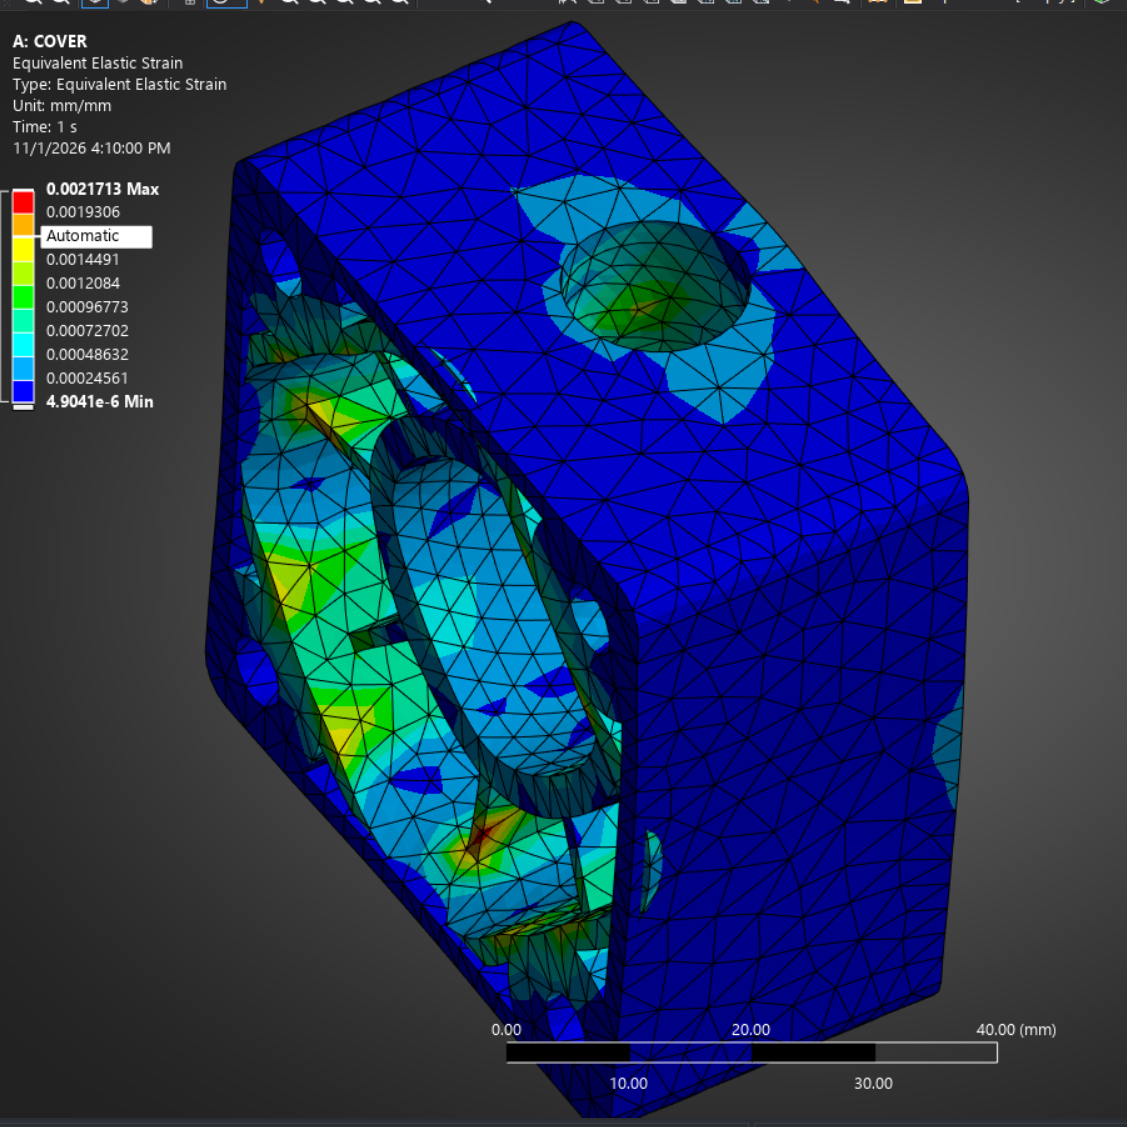
\includegraphics[width=\textwidth]{strain2.png}
				\caption{Mesh refinement around vehicle}
				\label{fig:mesh}
			\end{subfigure}
			
			\vspace{0.5cm} % Adds vertical space between the rows
			
			% Bottom Left Image
			\begin{subfigure}[b]{0.48\textwidth}
				\centering
				%\includegraphics[width=\textwidth]{velocity_contour.png}
				\caption{Velocity contours and stagnation point}
				\label{fig:contour}
			\end{subfigure}
			\hfill
			% Bottom Right Image
			\begin{subfigure}[b]{0.48\textwidth}
				\centering
				%\includegraphics[width=\textwidth]{streamlines_wake.png}
				\caption{Streamlines and wake region}
				\label{fig:wake}
			\end{subfigure}
			
			\caption{ANSYS CFD simulation Strain .}
			\label{fig:all_results}
			
		\end{figure}
		
	
	
	
	
	%%%%%%%%%%%%%%%%%%%%%%%%%%%%%%%%%%%%%%%%%%%%%%%%%%%%%%%%%%%%%%%%%%%%%%%%%%%%%%%%%%%%%%%%%%%%%%%%%%%%%%%%%%%%%%%%%%%%%%%%
	
	%%%%%%%%%%%%%%%%%%%%%%%%%%%%%%%%%%%%%%%%%%%%%%%%%%%%%%%%%%%%%%%%%%%%%%%%%%%%%%%%%%%%%%%%%%%%%%%%%%%%%%%%%%%%%%%%%%%%%%%%
	
		\newpage
	
	% -----------------------------------------------------------------
	\section{Conclusion}
	% -----------------------------------------------------------------
	The FEA simulation in ANSYS successfully identified the critical areas of the part under load. Results show a maximum stress of $185.4\text{ MPa}$ located at the fillet, yielding a factor of safety of $1.35$.
	
\end{document}














%%%%%%%%%%%%%%%%%%%%%%%%%%%%%%%%%%%%%%%%%%%%%%%%%%%%%%%%%%%%%%%%%%%%%%%%%%%%%%%%%%%%%%%%%%%%%%%%%%%%%%%%%%%%%%%%%%%%%%%%

%%%%%%%%%%%%%%%%%%%%%%%%%%%%%%%%%%%%%%%%%%%%%%%%%%%%%%%%%%%%%%%%%%%%%%%%%%%%%%%%%%%%%%%%%%%%%%%%%%%%%%%%%%%%%%%%%%%%%%%%




%%%%%%%%%%%%%%%%%%%%%%%%%%%%%%%%%%%%%%%%%%%%%%%%%%%%%%%%%%%%%%%%%%%%%%%%%%%%%%%%%%%%%%%%%%%%%%%%%%%%%%%%%%%%%%%%%%%%%%%%

%%%%%%%%%%%%%%%%%%%%%%%%%%%%%%%%%%%%%%%%%%%%%%%%%%%%%%%%%%%%%%%%%%%%%%%%%%%%%%%%%%%%%%%%%%%%%%%%%%%%%%%%%%%%%%%%%%%%%%%%





%%%%%%%%%%%%%%%%%%%%%%%%%%%%%%%%%%%%%%%%%%%%%%%%%%%%%%%%%%%%%%%%%%%%%%%%%%%%%%%%%%%%%%%%%%%%%%%%%%%%%%%%%%%%%%%%%%%%%%%%

%%%%%%%%%%%%%%%%%%%%%%%%%%%%%%%%%%%%%%%%%%%%%%%%%%%%%%%%%%%%%%%%%%%%%%%%%%%%%%%%%%%%%%%%%%%%%%%%%%%%%%%%%%%%%%%%%%%%%%%%                  